\documentclass{cmspaper}
\usepackage{graphicx}
\usepackage{amsmath}
\usepackage{amssymb}
\usepackage{subfigure}
\usepackage{multirow}
\usepackage[pdfborder=0 0 0,
            colorlinks,
            urlcolor = blue,
            linkcolor = black,
            citecolor = black,
            menucolor = black,]
           {hyperref}
%% \usepackage[colorlinks]{hyperref}
%% \usepackage{url}
\usepackage[toc,page]{appendix}
\renewcommand{\appendixname}{Appendix}
%% \renewcommand{\appendixtocname}{List of appendices}

% % useful definitions

% processes
\def\dyee {\ensuremath{Z/\gamma^*\to ee}}
\def\dymm {\ensuremath{Z/\gamma^*\to\mu\mu}}
\def\dytt {\ensuremath{Z/\gamma^*\to\tau\tau}}
\def\zee {\ensuremath{Z\to ee}}
\def\zmm {\ensuremath{Z\to\mu\mu}}
\def\ztt {\ensuremath{Z\to\tau\tau}}
\def\ttbar {\ensuremath{t\bar{t}}}
\def\wwll {\ensuremath{WW\to l^+l^-}}
\def\wwlulu{\ensuremath{WW\to l^+\nu l^-\bar{\nu}}}
\def\ww {\ensuremath{WW}}
\def\wz{\ensuremath{WZ}}
\def\zz{\ensuremath{ZZ}}
\def\wgamma{\ensuremath{W\gamma}}
\def\wjets{\ensuremath{W+}jets} 
\def\tw{\ensuremath{tW}} 
\def\singletopt{\ensuremath{t} ($t$-chan)} 
\def\singletops{\ensuremath{t} ($s$-chan)} 
\def\all{all}
\def\ee{\ensuremath{ee}}
\def\emu{\ensuremath{e\mu}}
\def\mm{\ensuremath{\mu\mu}}

%units

%others
\def\pt{\ensuremath{p_T}}
\def\ipb{pb\ensuremath{^{-1}}}
\def\ifb{fb\ensuremath{^{-1}}}
\def\et{\ensuremath{E_T}}
\def\met{\ensuremath{E\!\!\!\!/_T}}
\def\fBrem{\ensuremath{f_{\rm brem}}}
\def\pin{\ensuremath{p_{\rm in}}}
\def\pout{\ensuremath{p_{\rm out}}}

\input{commands}
\newcommand{\met}{\mbox{$E_T\hspace{-1.1em}/$\hspace{0.7em}}}

\setcounter{topnumber}{1}
\setcounter{bottomnumber}{1}


\begin{document}
\begin{titlepage}

\analysisnote{2011/489}

\date{\today}

\title{Matrix Element based searches for Standard Model Higgs boson in di-lepton final states with Full 2011 dataset.}

\begin{Authlist}
%
W.~Andrews~\Aref{ 4 }, 
D.~Barge~\Aref{ 3 }, 
L.~Bauerdick~\Aref{ 1 }, 
G.~Bauer~\Aref{ 2 },
J.~Bendavid~\Aref{ 2 },
I.~Bloch~\Aref{ 1 }, 
K.~Burkett~\Aref{ 1 }, 
E.~Butz~\Aref{ 2 },
C.~Campagnari~\Aref{ 3 }, 
G.~Cerati~\Aref{ 4 },
M.~Chan~\Aref{ 2 },
V.~Dutta~\Aref{ 2 },
D.~Evans~\Aref{ 4 }, 
P.~Everaerts~\Aref{ 2 },
I.~Fisk~\Aref{ 1 }, 
G.~G\'omez-Ceballos~\Aref{ 2 },
Y.~Gao~\Aref{ 1 }, 
F.~Golf~\Aref{ 4 }, 
M.~Goncharov~\Aref{ 2 },
O.~Gutsche~\Aref{ 1 }, 
K.~Hahn~\Aref{ 2 },
P.~Harris~\Aref{ 2 },
B.~Hooberman~\Aref{ 1 },
S.~Jindariani~\Aref{ 1 },
P.~Kalavase~\Aref{ 3 }, 
M.~Klute~\Aref{ 2 },
D.~Kovalskyi~\Aref{ 3 }~\Aref{ 6 }, 
I.~Kravchenko~\Aref{ 5 },
V.~Krutelyov~\Aref{ 3 }, 
I.~MacNeill~\Aref{ 4 },
S.~Nahn~\Aref{ 2 },
S.~Padhi~\Aref{ 4 }, 
C.~Paus~\Aref{ 2 },
D.~Ralph~\Aref{ 2 },
J.~Ribnik~\Aref{ 3 },
M.~Rudolph~\Aref{ 2 },
F.~Stoeckli~\Aref{ 2 },
K.~Sumorok~\Aref{ 2 },
K.~Sung~\Aref{ 2 },
S.~Tkaczyk~\Aref{ 1 },
Y.~Tu~\Aref{ 4 }, 
F.~W\"urthwein~\Aref{ 4 }, 
R.~Wolf~\Aref{ 2 },
S.~Xie~\Aref{ 2 },
A.~Yagil~\Aref{ 4 }, 
M.~Yang~\Aref{ 2 },
J.~Yoo~\Aref{ 4 },
M.~Zanetti~\Aref{ 2 }
%
\end{Authlist}
\Anotfoot{ 1 }{Fermilab National Accelerator Laboratory, Batavia, USA}
\Anotfoot{ 2 }{Laboratory for Nuclear Science, Massachusetts Institute of Technology, Cambridge, USA}
\Anotfoot{ 3 }{University of California, Santa Barbara, Santa Barbara, USA}
\Anotfoot{ 4 }{University of California, San Diego, San Diego, USA}
\Anotfoot{ 5 }{University of Nebraska-Lincoln, USA}
\Anotfoot{ 6 }{CERN, Switzerland}

\begin{abstract}
In this note we present searches for the standard model Higgs boson in the $WW \rightarrow l^{+}l^{-}\nu\bar{\nu}$ and $ZZ \rightarrow l^{+}l^{-}\nu\bar{\nu}$ 
final states. To achieve improved sensitivity compared to a cut-based approach, we use event probabilities based on Standard Model matrix elements to construct a likelihood function of the Higgs content of the data sample. The $H\rightarrow WW$ and $H\rightarrow ZZ$ analyses are performed using data sample corresponding to an integrated luminosity of 4.7 $fb^{-1}$  from $pp$ collisions at $\sqrt{s}=7$ TeV.
Events are required to have two reconstructed leptons, muons or electrons. For the $H\rightarrow WW$ search we compare the performance of the 
Matrix Element method to cut-based and Boosted Decision Tree based approaches. For the $H\rightarrow ZZ$ search we compare its performance to cut-and-count analysis and $m_{T}$ shape based one. We demonstrate that, with all systematic uncertainties taken into account, use of the matrix element method leads to a $15-30 \%$ improvement in the sensitivity when compared to cut-and-count based approach in both analyses. When compared to other shape analyses, it gives performance similar to that of the BDT in $H\rightarrow WW$, and performs 10\% better than $m_{T}$ at 250-300 GeV Higgs mass in $H\rightarrow ZZ$, with equal to $m_{T}$ performance at higher masses. Overall, using full 2011 4.7 $fb^{-1}$ data sample, we exclude Standard Model Higgs boson with mass 128--270 GeV (in $H\rightarrow WW$) and 310--500 GeV (in $H\rightarrow ZZ$) at 95\% C.L. 
\end{abstract}

%\maketitle

\end{titlepage}
\tableofcontents
%\listoftables
%\listoffigures
\newpage 

% body of paper here - Use proper section commands
% References should be done using the \cite, \ref, and \label commands

\section{Introduction}
\label{sec:Intro}
The Standard Model (SM) of elementary particles describes a universe in which fermions, the fundamental 
constituents of  matter, interact via fundamental forces propagated by gauge bosons. This description of elementary
particles and their interactions has been validated extensively through precision experiments and found to be incredibly
successful at describing the particle physics world. However, experimentally, there remains a missing piece of the
puzzle yet to be observed.  The SM incorporates a mechanism for symmetry breaking, known as the Higgs mechanism 
\cite{ref:HiggsMechanism,ref:HiggsMechanism1}, which naturally predicts the massive W and Z bosons as propagators of the weak 
force and provides a mechanism through which leptons and quarks are also able to acquire mass. An additional consequence of 
the Higgs mechanism is the existence of an associated massive scalar boson known as the Higgs boson, which is the only unobserved particle within
the SM framework.  Because of the central role of the Higgs mechanism in the SM, the discovery (or non-discovery) of the
Higgs boson along with additional studies of its properties will either confirm the current model or point toward new physics 
processes at the TeV energy scale.

The SM postulates the existence of the Higgs boson, but does predict its mass, which is a free parameter in the model. 
However, experimental measurements provide constraints on the Higgs mass.  Global fits to precision electroweak measurements 
set a one-sided 95$\%$ confidence level upper limit on Higgs boson mass at 157 \GeVcc \cite{ref:GlobalEwkConstraints}.
These constraints are mostly driven by measurements of the top quark and $W$ boson masses. Moreover, direct searches
at LEP have excluded a Higgs boson with mass below $114.4$ \GeVcc at 95$\%$ confidence level \cite{ref:LepExclusion}, and the Tevatron
has reported a preliminary update which extends the exclusion region for a Higgs boson mass between 156 and 177 \GeVcc \cite{ref:TevExclusion}.
Therefore, probing the mass range between 115 and 200 \GeVcc is crucial for Higgs boson searches.

Regardless of the mass, the dominant mechanism for production of the Higgs boson is gluon fusion (GF)\cite{ref:GF1,ref:GF2}, where the Higgs
is produced from a pair of gluons via a quark (primarily top-quark) loop. Another production mechanism is vector boson 
fusion (VBF) \cite{ref:VBF}, where the Higgs boson is produced from a pair of $W$ or $Z$ bosons. The relative contributions of GF and VBF
to the total Higgs boson production rate depend on the mass, but are approximately 90$\%$ and 10$\%$ over the range allowed
by electroweak constraints.  The Higgs boson can also be produced via associated production \cite{ref:VH1,ref:VH2} and top-quark fusion, however
contributions from these processes in the range of interest are small.

The Higgs decay mode is mostly determined by its mass \cite{ref:Hdecay}. While the diphoton decay channel dominates at low masses, searches 
in this channel face complications arising from large backgrounds and require excellent understanding of the electromagnetic
calorimeter response. For a SM Higgs boson mass $m_{H}>125$ GeV the $WW$ decay channel dominates and provides the opportunity of observing a 
Higgs signal in a wide range of masses between 120 and 300 \GeVcc.  The fully leptonic final state $H \rightarrow WW 
\rightarrow l^{+}l^{-}\nu\bar{\nu}$ provides a clean dilepton signature that is relatively easy to trigger on and has lower backgrounds compared to
semi-leptonic and hadronic final states. With a large signal yield and manageable backgrounds, 
this final state is the most promising discovery channel from early CMS data. 

The backgrounds in the $H \rightarrow WW \rightarrow l^{+}l^{-}\nu\bar{\nu}$ search are diboson production ($WW$, $WZ$ and $ZZ$), top-pair and 
single-top production, $W+$jet production where a hadronic jet fakes the signature of a lepton, $W+\gamma$ where a photon 
converts and produces a pair of electrons, one of which is not reconstructed, and Drell-Yan processes.  The most significant are
non-resonant $WW$ production and $W+$~jets.

While current fits to electroweak parameters prefer a low mass Higgs boson, the presence of non-SM physics at a higher mass scale can significantly alter
 the constraints. A search for the SM Higgs boson in the $H \rightarrow ZZ \rightarrow l^{+}l^{-}\nu\bar{\nu}$ final state provides sensitivity over the large
range of Higgs masses from 250 to 600 \GeVcc. The background in this mode is coming primarily from diboson processes as well as from Drell-Yan events with fake missing transverse energy due to the lepton/jet energy and direction mis-measurements. 

In this note we present a search for the standard model Higgs boson in the $WW \rightarrow ll\nu\bar{\nu}$ and $ZZ \rightarrow ll\nu\bar{\nu}$ final states 
using a Matrix Element (ME)-based discriminant. Triggers, event pre-selection, and reconstruction of high level objects are described 
in detail in notes \cite{ref:HWW2011smurf}, \cite{ref:HZZ2011smurf} and references within. Here, we introduce the ME technique, 
describe its technical implementation, summarize the event selection, present results and compare them to the ones obtained with 
other methods. The reader is first introduced to the method using the $H\rightarrow WW \rightarrow ll\nu\bar{\nu}$ search; the
$H \rightarrow ZZ \rightarrow ll\nu\bar{\nu}$ search is then described in a subsequent section without repeating details common to the two analyses.



\section{$H \rightarrow WW$ }

\subsection{Method Overview}
\label{sec:Meth_Overview}
\label{hwwintro}

\subsection{Event Probability}
\label{sec:Evt_Prob}
\subsubsection{General Considerations}
The Matrix Element method relies on the evaluation of the event probability densities for the signal and background processes based on the 
standard model differential cross-section calculation. 

In general, a differential cross-section is given by \cite{ref:PDG}:
\begin{equation}
d\sigma=\frac{(2\pi)^{4} \left| M \right|^{2}}{4\sqrt{(q_{1}q_{2})^{2}-m_{q_{1}}^{2}m_{q_{2}}^{2}}}d\Phi_{n}(q_{1}+q_{2};p_{1},...p_{n}),
\label{eqn:DiffXsecGeneral}  
\end{equation}
where $\left| M \right|$ is the Lorentz invariant matrix element;
$q_{1}$,$q_{2}$ and $m_{q_{1}}$,$m_{q_{2}}$ are the four momenta and masses of the incident particles 
(in our case quarks or gluons), 
$p_i$ is the four momentum of the $i-$th outgoing particle, 
and $d\Phi_{n}$ is the $n$-body phase space given by:
\begin{equation}
d\Phi_{n}(q_{1}+q_{2};p_{1},...p_{n})=\delta^{4}(q_{1}+q_{2}-\sum_{i=1}^{n}{p_{i}})\prod\frac{d^{3}p_{i}}{(2\pi)^{3}2E_{i}}.
\label{eqn:PhaseSpaceGeneral}  
\end{equation}
where the sum runs over the $n$ outgoing particles produced in the collision.
It is important to note here that energies of the incident partons are not known and are distributed according to the parton density 
functions (PDFs). Therefore, for a certain set of observed kinematic properties $x$, one can write the probability of observing it as:
\begin{equation}
P(x)=\frac{1}{\sigma}\int d\sigma(y)dq_{1}dq_{2}f(y_{1})f(y_{2})W(x;y),
\label{eqn:EvtProbGeneral}  
\end{equation}
where $y=(p_{1}...p_{n})$ is the set of parton level variables needed to describe an event, $d\sigma(y)$ is the differential cross-section 
in terms of $y$, $f(y_{1})$ and $f(y_{2})$ are the PDFs and $W(x;y)$ is a transfer function which maps parton level quantities to the 
reconstructed quantities.  One can think of $W(x;y)$ as the probability of observing a reconstructed event $x$ given an event with parton level properties $y$. $\sigma$ is a normalization constant which is discussed separately below.

Assuming that  the momenta of the incident partons have no transverse component, the four vectors can be written as:
\begin{equation}
q_{1}=(0,0,\xi_{1}E_{beam},\xi_{1}E_{beam}),
q_{2}=(0,0,-\xi_{2}E_{beam},\xi_{2}E_{beam}),
\label{eqn:EvtProbGeneral2}  
\end{equation}
where $\xi_{1}$ and $\xi_{2}$ are fractions of the proton energy carried by the initial partons as given by the PDFs, and
$E_{beam}=3.5$ TeV. Assuming that the initial state partons are massles, we can rewrite the ``flux'' term:
\begin{equation}
\frac{1}{\sqrt{(q_{1}q_{2})^{2}-m_{q_{1}}^{2}m_{q_{2}}^{2}}} \approx \frac{1}{2 E_{q_{1}}E_{q_{2}}}.
\label{eqn:flux}  
\end{equation}
where $E_{q_{i}} = \xi_i\times E_{beam}$.  
Taking into account Eq.~\ref{eqn:DiffXsecGeneral} and \ref{eqn:PhaseSpaceGeneral}, and considering final states with four particles,
Eq.~\ref{eqn:EvtProbGeneral} can be re-written as:
\begin{equation}
P(x)=\frac{1}{ \sigma}\int 2 \pi^{4} \left| M \right|^{2} \frac{f(y_{1})f(y_{2})}{(E_{q_{1}}E_{q_{2}})^{2}}W(x;y)d\Phi_{4}dE_{q_{1}}dE_{q_{2}},
\label{eqn:EvtProbGeneral3}  
\end{equation}
or
\begin{equation}
P(x)=\frac{1}{\sigma }\int 2 \pi^{4} \left| M \right|^{2} \frac{f(\xi_{1})f(\xi_{2})}{\xi_{1}\xi_{2}E_{beam}^{2}}W(x;y)d\Phi_{4}d\xi_{1}d\xi_{2},
\label{eqn:EvtProbGeneral4}  
\end{equation}

\subsubsection{Normalization Constant}
If the integration is performed over the entire kinematic phase space, then the normalization term $\sigma$ is equal
to the total cross-section $\sigma_{total}$.  However, if the integration is performed only over the acceptance region,
then $\sigma=A\sigma_{total}$, where $A$ is the acceptance term for a given physics process, or in other words the fraction
of the total cross-section falling into the acceptance region.  The acceptance term $A$ can be derived as:
\begin{equation}
A=\frac{N_{accepted}}{\sigma_{total}\times L},
\label{eqn:Acceptance}  
\end{equation}
where $N_{accepted}$ is the expected yield of events passing the acceptance selection, and $L$ is the integrated luminosity.

\subsubsection{Effect of the system boost}
Equation \ref{eqn:EvtProbGeneral3} is derived assuming no transverse component of the momenta of the incident partons,
which is true at Leading Order.   At next-to-leading order (NLO), however, initial state radiation (ISR) can generate a transverse momentum
of the system.  The distribution of the system transverse momentum depends on the amount of ISR and its $p_{T}$ spectrum, and
therefore may vary for different physics processes. In the presence of a transverse boost, the general probability expression can
be rewritten as:
\begin{equation}
P(x)=\frac{1}{\sigma }\int 2 \pi^{4} \left| M \right|^{2} \frac{f(\xi_{1})f(\xi_{2})}{\xi_{1}\xi_{2}E_{beam}^{2}}\epsilon(y)G(x;y)d\Phi_{4}d\xi_{1}d\xi_{2}K(k_{x},k_{y})dk_{x}dk_{y},
\label{eqn:EvtProbGeneralWithBoost}  
\end{equation}
where $K(k_{x},k_{y})$ is the transverse momentum distribution and $W(x;y)=\epsilon(y)G(x;y)$ is factorized into a reconstruction 
efficiency term $\epsilon(y)$ and a resolution function $G(x,y)$ accounting for detector resolution effects.
The efficiency and transfer functions are described in more detail in Sec.~\ref{sec:EfficiencyTransfer}.

\subsubsection{$l^{+}l^{-}\nu\bar{\nu}$ final state }
For the Higgs to $WW$ leptonic final state, $H \rightarrow WW \rightarrow l^{+}l^{-}\nu\bar{\nu}$, assuming no jet activity, 
the set of reconstructed quantities can be written as $x=(\vec{p}_{l1},\vec{p}_{l2}, \met_{x},  \met_{y})$.
The complication of this state is that it is not fully reconstructed, and information about the $z$-components of the neutrino 
momenta as well as individual neutrino transverse components are missing. It is, therefore, necessary to integrate over these 
unknown quantities. Expression \ref{eqn:EvtProbGeneralWithBoost} for this case can be written as:
\begin{eqnarray}
P(x)=\frac{1}{\sigma }\int 2 \pi^{4} \left| M \right|^{2} \frac{f(\xi_{1})f(\xi_{2})}{\xi_{1}\xi_{2}E_{beam}^{2}}
\epsilon(\vec{p}_{l1})\epsilon(\vec{p}_{l1}) \times \nonumber \\ 
                         G(p_{l1},p_{l2}, \met_{x},  \met_{y}; q_{l1}, q_{l2}, p_{\nu_{1,x}}+  p_{\nu_{2,x}}, p_{\nu_{1,y}}+p_{\nu_{2,y}})d\Phi_{4}d\xi_{1}d\xi_{2} \times \nonumber \\
                         K(k_{x},k_{y})dk_{x}dk_{y}\delta(p_{\nu_{1,x}}+p_{\nu_{2,x}}-\met_{x})\delta(p_{\nu_{1,y}}+p_{\nu_{2,y}}-\met_{y}).
\label{eqn:EvtProbGeneralWithBoost2L2nu}  
\end{eqnarray}
where $q_{l1}$ and $q_{l2}$ are true momenta of the leptons.

\subsection{Evaluation of the Differential Cross-Section}

\subsubsection{Integration}
The evaluation of the differential cross section requires integration over the missing kinematic information in an event, such 
as the longitudinal components of neutrino momenta, as well as integration over allowed values of the transverse momentum
of the system.

We perform the integration using Monte Carlo techniques, in which we generate values of unknown quantities based on a set of
random numbers.  Monte Carlo calculations can be carried out using sets of random points picked from any arbitrary probability 
distribution. The choice of the underlying distribution obviously makes a difference to the efficiency of the method. In most cases,
Monte Carlo calculations carried out using uniform probability distributions give very poor estimates of high-dimensional integrals
and are not a useful method of approximation. 
Therefore, we employ the algorithm of ``importance sampling'' in the Monte Carlo integration. Instead of choosing points from a 
uniform distribution, they are chosen from a distribution which concentrates the points in the region of phase space where the 
value of the function being integrated is large.  For example,
\begin{equation}
\label{eqn:ImpSampling}
I=\int_{x_{1}}^{x_{2}} f(x)dx = \int_{a}^{b} \frac{f(x)}{g(x)}dx,
\end{equation}
where the function $g(x)$ is chosen to be a reasonable approximation to $f(x)$. The integral can be calculated by choosing the random points 
from the probability distribution $g(x)$ and evaluating $f(x)/g(x)$ at these points.  Sampling from a non-uniform distribution for this function 
is more efficient than doing a crude Monte Carlo calculation without importance sampling.

The number of integration variables depends on the process for which the differential cross-section is evaluated. For example,
in the case of the gluon fusion signal there are four missing components of the neutrino momenta,
$(\nu_{x}, \nu_{y}, \nu_{z}, \bar{\nu}_{z})$, after including the $x$ and $y$~components of the $\met$.  
These quantities, in addition to the measured ones and also the two components of the transverse boost 
($k_{x}$ and $k_{y}$), fully define the system.
However, integration using  $(\nu_{x}, \nu_{y}, \nu_{z}, \bar{\nu}_{z})$ as the set of variables is not efficient.  Due to the narrow 
Breit-Wigner width of the Higgs and $W$ bosons, most points chosen at random from a uniform distribution will lie outside of 
the core of the cross-section function. To avoid this and improve the
efficiency of the integration, we perform the variable transformations 
$\nu_{x} \rightarrow m_{H}^{2}$ and $\nu_{y} \rightarrow m_{W}^{2}$ 
so that the set of integration variables becomes $(m_{H}^{2}, m_{W}^{2}, \nu_{z}, \bar{\nu}_{z})$.
A Jacobian corresponding to the transformation is calculated analytically and properly 
accounted for. The integration is then performed using the importance sampling method, with neutrino $z$-components sampled
using an exponential function and $m_{H}^{2}$ and $m_{W}^{2}$ using narrow Breit-Wigner distributions.
Similarly, for non-resonant $WW$ production, the set of variables used for the integration is:
$(m_{W1}^{2}, m_{W2}^{2}, \nu_{z}, \bar{\nu}_{z})$. In the $W$+jet case, there is only one missing quantity $\nu_{z}$ which is sampled using 
an exponentially falling function.

For each event we perform 100,000 integration steps. To verify that this is sufficient, for randomly selected events we calculate differential cross
sections using 500,000 integration steps and compare them to the ones obtained with 100,000. In the vast majority of cases the difference
was $< 1\%$ and the largest observed deviation was $\sim 5\%$. 

\subsubsection{Comparison of Differential Cross Section for Signal and Background Events}

Integration over the event-by-event differential cross-section $\frac{d\sigma}{dx}$ is used to evaluate the probability $P$ as described
in Equation~\ref{eqn:EvtProbGeneral}.  Since we expect to see different probabilities for signal and background events,
we should see separation in the differential cross-sections for different signal and
background processes when looking at the same events.  For now we restrict our comparison to just the signal,
$H\rightarrow WW$, and the dominant background, non-resonant $WW$ production.

Figure~\ref{subfig:HWWXsec} shows the differential cross section for gluon fusion Higgs production,
$d\sigma(H \rightarrow WW)/dx$, calculated for gluon fusion Higgs signal events and for non-resonant $WW$ events.
The distribution for signal events is shifted to larger values of  $d\sigma(H \rightarrow WW)/dx$ compared to that
of non-resonant $WW$, and it has a narrower width. 
Figure~\ref{subfig:HWWXsecvsdPhi} shows the distribution of $d\sigma(H \rightarrow WW)/dx$ as a function of
$\Delta\phi_{ll}$ for signal and non-resonant $WW$ events.
As described in Sec.~\ref{sec:Meth_Overview}, the distributions of $\Delta\phi_{ll}$ are different for the signal and the $WW$
background due to spin effects. We see here that the differential cross-section is correlated with $\Delta\phi_{ll}$ and is on average decreasing with
increasing azimuthal angle, since the signal will be concentrated at smaller values of $\Delta\phi_{ll}$.
Figure~\ref{subfig:Xsec_WWvsHWW} shows distributions of these events in the $d\sigma(H \rightarrow WW)/dx$ 
vs. $d\sigma(WW)/dx$ plane. One can see that while a certain level of separation can be achieved, there is a 
non-negligible overlapping region of phase space where events from the two processes are indistinguishable.
%Finally, figure~\ref{subfig:to be inserted} shows distributions of signal and $W$+jet 
%events in $d\sigma(H \rightarrow WW)/dx$ vs $d\sigma(W+jet)/dx$ plane (this one needs to be made and inserted).

\begin{figure}[!hbtp]                                                                                         
\centering                                                                                                    
\subfigure[]{                                                                                                 
\centering                                                                                                    
\label{subfig:HWWXsec}                                                                                       
\includegraphics[width=.42\textwidth]{figures/HWWXsec.png}}                                                                                       
\subfigure[]{                                                                                                 
\centering                                                                                                    
\label{subfig:HWWXsecvsdPhi}                                                                                       
\includegraphics[width=.42\textwidth]{figures/HWWXsecvsdPhi.png}}                                            
\subfigure[]{                                                                                                 
\centering                                                                                                    
\label{subfig:Xsec_WWvsHWW}                                                                                       
\includegraphics[width=.42\textwidth]{figures/Xsec_WWvsHWW.png}}\\                                            
\caption{Distributions of \subref{subfig:HWWXsec} the differential cross-section, $d\sigma(H \rightarrow WW)/dx$, 
\subref{subfig:HWWXsecvsdPhi} differential cross-section vs. $\Delta\phi_{ll}$, and 
\subref{subfig:Xsec_WWvsHWW}  $d\sigma(H \rightarrow WW)/dx$ vs. $d\sigma(WW)/dx$, 
for simulated Higgs signal and non-resonant $WW$ events.}
\label{fig:dXsecPlots}                                                                                          
\end{figure}                      

\subsubsection{$k_{T}$ Functions} 
In the leading order Matrix Element calculation there is no initial state radiation. The initial state partons 
collide head-on and the system has no transverse boost. To account for the transverse recoil and thus improve the performance 
of our discriminant on data, we integrate over the possible values of the system boost $K(k_x,k_y)$. The $K(k_x,k_y)$ model
is extracted from Monte Carlo for each process separately. Figure~\ref{fig:wwboost} shows a comparison of the distributions
of transverse boost for gluon fusion Higgs production at three different values of $m_H$ and the 
non-resonant $W^{+}W^{-}$ process.

\begin{figure}[!htbp]                                                                                         
\begin{center}                                                                                                
\includegraphics[width=0.5\textwidth]{figures/boost.pdf}                                                      
\caption{The transverse boost of the $WW$ system for $WW$ production and $H \rightarrow WW$ at 3 different Higgs masses.} 
\label{fig:wwboost}                                                                                           
\end{center}                                                                                                  
\end{figure}    

The effect of accounting for the transverse boost of the $WW$ system in the calculations of the differential cross-section
is demonstrated in Figure~\ref{fig:kteffect}. In the absence of the boost, there is a tail in the differential cross-section distribution
for Higgs signal events, with some events having small values of $d\sigma(H \rightarrow WW)/dx$.  
These events would likely be classified as background-like. Accounting for the system boost removes this tail,
allowing for better signal and background discrimination. 

\begin{figure}[!hbtp]                                                                                         
\centering                                                                                                                                             
\includegraphics[width=.84\textwidth]{figures/SystemBoostEffect.png}\\                                            
\caption{
Distributions of the differential cross-section, $d\sigma(H \rightarrow WW)/dx$ for simulated Higgs signal and non-resonant $WW$ events
(a)using no system boost $K$, and (b) including a system boost.}
\label{fig:kteffect}                                                                                          
\end{figure}          

\subsection{Probability Calculations and Likelihood Ratio}
\label{sec:Probability}
The evaluation of the event probability was described in Sec.~\ref{sec:Evt_Prob} and 
Eq.~\ref{eqn:EvtProbGeneralWithBoost}~and~\ref{eqn:EvtProbGeneralWithBoost2L2nu}.
Two components of the determination of the event probability are the efficiency
and transfer functions described in detail here.

\subsubsection{Efficiency and Transfer Functions}
\label{sec:EfficiencyTransfer}
The efficiency functions $\epsilon(\vec{p})$ provide the probability that a lepton of given momentum
will be reconstructed in the detector. We evaluate this probability using non-resonant $q\bar{q}\rightarrow WW$
separately for muons and electrons and parametrize the probability as a function of the reconstructed
lepton $p_{T}$ and $\eta$.
The probability in each ($p_{T}$,$\eta$) bin is defined as the number of fully reconstructed leptons divided 
by the number of generator level leptons. Figure~\ref{fig:lepeff_gen} shows the 
one dimensional projection of the efficiency as a function of the lepton $\eta$ and $p_{T}$, separately for
muons and electrons. 
A scale factor to account for differences between 
data and Monte Carlo can be calculated using a tag-and-probe analysis and applied when calculating event 
probabilities for data events.

\begin{figure}[!htbp]
\begin{center}
\includegraphics[width=0.4\textwidth]{figures/lepton_eff_Eta.pdf}
\includegraphics[width=0.4\textwidth]{figures/lepton_eff_Pt.pdf}\\
\caption{Lepton efficiency as a function of the lepton $\eta$ (left) and $p_{T}$ (right) extracted 
from the $WW$ Monte Carlo.}
\label{fig:lepeff_gen}
\end{center}
\end{figure}

Transfer functions $G(x;y)$ provide the probability of measuring the set of reconstructed variables ($x$) originating 
from a set of production variables ($y$). 
The general idea of these functions is to introduce a relation between the kinematic properties of parton-level objects
and reconstructed objects.
The set ($y$) represents the final state charged lepton and neutrino momenta at
the particle level, while the set ($x$) represents the measured lepton momenta and $\met$ in the CMS
detector. 
In the case of well-measured objects, such as lepton momenta, it is assumed that the reconstructed quantity is equal
to the generator level quantity.  The transfer function $G(x;y)$ is then considered to be a $\delta$-function, and the 
reconstructed lepton momenta are used in the differential cross-section calculations. For unmeasured quantities, such as
the longitudinal component of the neutrino momenta, the transfer function is unity. The sum of the transverse components
of the neutrino momenta can be inferred from energy and momentum conservation.

\subsubsection{Fake Leptons}
\label{sec:FakeLeptons}
The determination of the event probability for $W$+jet events must be handled slightly differently from other processes.
For these events to be reconstructed in the dilepton final state, one of the identified reconstructed leptons has been
faked by a parton fragmenting and hadronizing into a QCD jet which then fakes the signature of a lepton in the detector. 
To account for this effect properly, we multiply the differential cross-section for the $W$+jet process by the 
probability for a parton to be reconstructed as a lepton with the measured kinematics. This probability can be 
factorized into two terms:
\begin{eqnarray}
\begin{array}{lcl}
P(parton\rightarrow lepton)=P(parton\rightarrow FO) \times P(FO\rightarrow lepton),
\end{array} 
\end{eqnarray} 
where FO refers to a so-called ``fakeable object''. The first term in the product is measured using Monte Carlo and 
parametrized in $p_{T}$ and $\eta$. The second term is the fake rate measured in the data. The values 
of $P(parton \rightarrow lepton)$ are illustrated in Figure~\ref{fig:lepgenfr} for electrons and muons.
In both cases, $P$ is in the range $10^{-3}-10^{-4}$.

We cross check $P(parton \rightarrow lepton)$ values that we obtain using this method by comparing them to values 
measured in a $\gamma$+jet Monte Carlo and data samples.  In Monte Carlo, we check that in both samples, $W$+jet and  $\gamma$+jet,
electron fakeable objects originate most frequently from light quarks while muon fakeable objects are coming primarily
from semi-leptonic decays of charm and bottom quarks, as shown in Figure~\ref{fig:fakeorigins}.
Then using  $\gamma$+jet events we calculate the probability as ratio of the number of fakeable objects and number of jets in each $\eta$ and $p_{T}$ bin.
Probabilities obtained using these two methods agree well within the uncertainty. 

It should be also noted that in most cases the momentum of a fake lepton is significantly smaller than that of the faking parton.
To account for this effect we use the transfer function to map the parton-level quark or gluon momentum to the reconstructed
momentum of the fake lepton.
We extract this function from Monte Carlo by matching status code 3 partons to fakeable objects within a
cone of $\Delta R=0.2$.
The function is parametrized in the $p_{T}$ of the fakeable object and is shown in Figure~\ref{fig:ptresponse}.
In principle, not only $p_{T}$ but also the direction of the parton can differ from the reconstructed direction of the fakeable object.
However, we find that in the vast majority of cases they lie within $\Delta R<0.1$, as shown in Figure~\ref{fig:partonleptondirection},
and the difference has very little effect on the results of the analysis. Therefore, we do not apply any corrections to the direction
of the parton.


\begin{figure}[!htbp]                                                                                         
\begin{center}                                                                                                
\includegraphics[width=0.4\textwidth]{figures/wjets_heleGenFR.pdf}                                            
\includegraphics[width=0.4\textwidth]{figures/wjets_hmuGenFR.pdf}\\                                           
\caption{The probability for a parton to pass the electron (left) and muon (right)                            
fakeable object selections. }                                                                                 
\label{fig:lepgenfr}                                                                                          
\end{center}                                                                                                  
\end{figure}   

\begin{figure}[!htbp]                                                                                         
\begin{center}                                                                                                
\includegraphics[width=0.9\textwidth]{figures/ElectronFakeOrigin.png}                                            
\includegraphics[width=0.9\textwidth]{figures/MuonFakeOrigin.png}\\                                           
\caption{ Origin of the electron and muon fakeable objects. The plot shows 
that electron fakes originate mostly from light quarks while muon fakes
are coming primarily from semi-leptonic heavy quark decays.}
\label{fig:fakeorigins}                                                                                          
\end{center}                                                                                                  
\end{figure}   


\begin{figure}[!htbp]                                                                                         
\begin{center}                                                                                                
\includegraphics[width=0.4\textwidth]{figures/ElectronPtResponse.png}                                            
\includegraphics[width=0.4\textwidth]{figures/MuonPtResponse.png}\\                                           
\caption{Ratio of transverse momentum of a fakeable object and parton transverse momentum
for electron (left) and muons (right). }                                                                                 
\label{fig:ptresponse}                                                                                          
\end{center}                                                                                                  
\end{figure}   

\begin{figure}[!htbp]                                                                                         
\begin{center}                                                                                                
\includegraphics[width=0.8\textwidth]{figures/PartonLeptonDIrection.png}                                            
\caption{Distance in pseudo-rapidity (left) and azimuthal angle (right)
between generator level parton and reconstructed fakeable object.}                                                                                 
\label{fig:partonleptondirection}                                                                                          
\end{center}                                                                                                  
\end{figure}   


\clearpage
\subsubsection{Final Discriminant: Likelihood Ratio}
\label{sec:LR}
The Matrix Element functions used in this analysis are obtained from MCFM v5.8.  
MCFM provides both LO, and NLO cross-section calculations for 
all relevant background and Higgs production processes in $pp$ collisions. In this analysis 
we use only the LO Matrix Element. In the future we plan to improve our discriminant 
by taking advantage of the NLO Matrix Element. The PDF set used in the event probability 
calculations is CTEQ 6.1M.

Construction of the most optimal discriminant would require calculation 
of event probabilities for each of the background processes. In reality, however, having 
probabilities for only the signal hypothesis and the primary backgrounds is sufficient to achieve 
the desired level of discrimination. In this analysis we calculate for each event the probabilities 
for gluon fusion Higgs boson production (ggH), non-resonant $q\bar{q}\rightarrow WW$ pair 
production (WW) and the $W$+jet process where a $W$ boson is produced in association
with one jet.   For ggH we calculate the event probability given a specific hypothesis for the
mass and width of the Higgs.

Event probabilities, calculated as described above, are used to construct 
a likelihood ratio (LR) discriminant, which we use in a one-dimensional template fit.  
The discriminator is defined as :
\begin{equation}
\label{eqn:LR}
LR = \frac { P_s} { P_s + \sum_i k_{bi} P_{bi}},
\end{equation}
where $P_s$ is the signal probability, $P_{bi}$ is the probability of background $i$, and 
 $k_{bi}$ is the relative ratio of expected contribution of each background after the pre-selection, satisfying $\sum k_{bi} =1$.
In our particular case of two background process hypothesis, Eq.~\ref{eqn:LR} reduces to:
\begin{equation}
\label{eqn:LRHWW}
LR = \frac { P_{HWW}} { P_{HWW} + k_{WW} P_{WW}+k_{W+jet} P_{W+jet}},
\end{equation}
The calculation of $P_{HWW}$ is a function of Higgs mass so that the likelihood ratio
shape depends on $m_H$. This is true for both signal and background templates of $LR$.

It is important to note that because the LR distribution is calculated the same way for data,
signal MC, and background MC, the fact that we use the LO Matrix Element and make certain 
approximations in the analytic calculation may result in less than optimal sensitivity, but
it does not introduce any biases.



\subsection{Results}
\label{results_hww}
In this section, we document the results on the upper-limits using shape analysis based on 
the matrix element output, described in Section~\ref{sec:LR}. 
%The matrix element output has been evaluated for 18 different values of $m_H$ between 115 and 600 \GeVcc.
Figure~\ref{fig:me_115_4700pb}-\ref{me_200_4700} shows the likelihood ratio distributions for $m_H$~=~115, 120, 130, 140, 160 and 200\GeVcc,               
corresponding to 4.7~fb$^{-1}$. 
Note that the majority of backgrounds peak near $LR~=~0$ while the signal peaks near $LR~=~1$.  
It was noted in Sec.~\ref{sec:EvtSelWW} that we apply a dilepton invariant mass requirement prior to constructing the likelihood ratio. 
Figure~\ref{fig:LR_noMll} shows the likelihood ratio distribution assuming $m_{H}=160$ \GeVcc without the invariant mass requirements.
One can see from the peak at $LR~=~0$ that the Matrix Element method successfully identifies high invariant mass events as background-like, so the cut is not essential. However, by applying the cut we lose less than $1\%$ of the signal and gain significantly in processing time needed for differential cross-section calculations.

%%%%%%%%%%%%%%%%%%%%%%%%%%%%%%%%%%%%%
\begin{figure}[!hbtp]                                                                                         
\centering                                                                                                                                             
\includegraphics[width=.5\textwidth]{figures/LR_noMll.png}\\                                            
\caption{The matrix element output LR distribution after $WW$ selection but prior to $m_{ll}$ cut                      
for $m_H$=160 \GeVcc}
\label{fig:LR_noMll}                                                                                          
\end{figure}
%%%%%%%%%%%%%%%%%%%%%%%%%%%%%%%%%%%%%




%%%%%%%%%%%%%%%%%%%%%%%%%%%%%%%%%%%%%
\begin{figure}[!hbtp]
\centering
\subfigure[$e\mu$ 0-Jet]{
\centering
\label{subfig:me_115_0j_of_4700pb}
\includegraphics[width=.40\textwidth]{figures/ME_mH115_0j_of_stack_lin.pdf}}
\subfigure[$ee$/$\mu\mu$ 0-Jet]{
\centering
\label{subfig:me_115_0j_sf_4700pb}
\includegraphics[width=.40\textwidth]{figures/ME_mH115_0j_sf_stack_lin.pdf}}
\subfigure[$e\mu$ 1-Jet]{
\centering
\label{subfig:me_115_1j_of_4700pb}
\includegraphics[width=.40\textwidth]{figures/ME_mH115_1j_of_stack_lin.pdf}}
\subfigure[$ee$/$\mu\mu$ 1-Jet]{
\centering
\label{subfig:me_115_1j_sf_4700pb}
\includegraphics[width=.40\textwidth]{figures/ME_mH115_1j_sf_stack_lin.pdf}}
\caption{
ME output for $m_H$=115 GeV corresponding to \intlumi:
0-jet OF \subref{subfig:me_115_0j_of_4700pb},
0-jet SF \subref{subfig:me_115_0j_sf_4700pb},
1-jet OF \subref{subfig:me_115_1j_of_4700pb},
1-jet SF \subref{subfig:me_115_1j_sf_4700pb}
.}
\label{fig:me_115_4700pb}
\end{figure}

\begin{figure}[!hbtp]
\centering
\subfigure[$e\mu$ 0-Jet]{
\centering
\label{subfig:me_120_0j_of_4700pb}
\includegraphics[width=.40\textwidth]{figures/ME_mH120_0j_of_stack_lin.pdf}}
\subfigure[$ee/\mu\mu$ 0-Jet]{
\centering
\label{subfig:me_120_0j_sf_4700pb}
\includegraphics[width=.40\textwidth]{figures/ME_mH120_0j_sf_stack_lin.pdf}}
\subfigure[$e\mu$ 1-Jet]{
\centering
\label{subfig:me_120_1j_of_4700pb}
\includegraphics[width=.40\textwidth]{figures/ME_mH120_1j_of_stack_lin.pdf}}
\subfigure[$ee/\mu\mu$ 1-Jet]{
\centering
\label{subfig:me_120_1j_sf_4700pb}
\includegraphics[width=.40\textwidth]{figures/ME_mH120_1j_sf_stack_lin.pdf}}
\caption{
ME output for $m_H$=120 GeV corresponding to \intlumi:
0-jet OF \subref{subfig:me_120_0j_of_4700pb},
0-jet SF \subref{subfig:me_120_0j_sf_4700pb},
1-jet OF \subref{subfig:me_120_1j_of_4700pb},
1-jet SF \subref{subfig:me_120_1j_sf_4700pb}
.}
\label{fig:me_120_4700pb}
\end{figure}
%%%%%%%%%%%%%%%%%%%%%%%%%%%%%%%%%%%%%

%%%%%%%%%%%%%%%%%%%%%%%%%%%%%%%%%%%%%
\begin{figure}[!hbtp]
\centering
\subfigure[$e\mu$ 0-Jet]{
\centering
\label{subfig:me_130_0j_of_4700pb}
\includegraphics[width=.40\textwidth]{figures/ME_mH130_0j_of_stack_lin.pdf}}
\subfigure[$ee/\mu\mu$ 0-Jet]{
\centering
\label{subfig:me_130_0j_sf_4700pb}
\includegraphics[width=.40\textwidth]{figures/ME_mH130_0j_sf_stack_lin.pdf}}
\subfigure[$e\mu$ 1-Jet]{
\centering
\label{subfig:me_130_1j_of_4700pb}
\includegraphics[width=.40\textwidth]{figures/ME_mH130_1j_of_stack_lin.pdf}}
\subfigure[$ee/\mu\mu$ 1-Jet]{
\centering
\label{subfig:me_130_1j_sf_4700pb}
\includegraphics[width=.40\textwidth]{figures/ME_mH130_1j_sf_stack_lin.pdf}}
\caption{
ME output for $m_H$=130 GeV corresponding to \intlumi:
0-jet OF \subref{subfig:me_130_0j_of_4700pb},
0-jet SF \subref{subfig:me_130_0j_sf_4700pb},
1-jet OF \subref{subfig:me_130_1j_of_4700pb},
1-jet SF \subref{subfig:me_130_1j_sf_4700pb}
.}
\label{fig:me_130_4700pb}
\end{figure}
%%%%%%%%%%%%%%%%%%%%%%%%%%%%%%%%%%%%%

%%%%%%%%%%%%%%%%%%%%%%%%%%%%%%%%%%%%%
\begin{figure}[!hbtp]
\centering
\subfigure[$e\mu$ 0-Jet]{
\centering
\label{subfig:me_140_0j_of_4700pb}
\includegraphics[width=.40\textwidth]{figures/ME_mH140_0j_of_stack_lin.pdf}}
\subfigure[$ee/\mu\mu$ 0-Jet]{
\centering
\label{subfig:me_140_0j_sf_4700pb}
\includegraphics[width=.40\textwidth]{figures/ME_mH140_0j_sf_stack_lin.pdf}}
\subfigure[$e\mu$ 1-Jet]{
\centering
\label{subfig:me_140_1j_of_4700pb}
\includegraphics[width=.40\textwidth]{figures/ME_mH140_1j_of_stack_lin.pdf}}
\subfigure[$ee/\mu\mu$ 1-Jet]{
\centering
\label{subfig:me_140_1j_sf_4700pb}
\includegraphics[width=.40\textwidth]{figures/ME_mH140_1j_sf_stack_lin.pdf}}
\caption{
ME output for $m_H$=140 GeV corresponding to \intlumi:
0-jet OF \subref{subfig:me_140_0j_of_4700pb},
0-jet SF \subref{subfig:me_140_0j_sf_4700pb},
1-jet OF \subref{subfig:me_140_1j_of_4700pb},
1-jet SF \subref{subfig:me_140_1j_sf_4700pb}
.}
\label{fig:me_140_4700pb}
\end{figure}
%%%%%%%%%%%%%%%%%%%%%%%%%%%%%%%%%%%%%


              
%%%%%%%%%%%%%%%%%%%%%%%%%%%%%%%%%%%%%
\begin{figure}[!hbtp]
\centering
\subfigure[$e\mu$ 0-Jet]{
\centering
\label{subfig:me_160_0j_of_4700pb}
\includegraphics[width=.40\textwidth]{figures/ME_mH160_0j_of_stack_lin.pdf}}
\subfigure[$ee/\mu\mu$ 0-Jet]{
\centering
\label{subfig:me_160_0j_sf_4700pb}
\includegraphics[width=.40\textwidth]{figures/ME_mH160_0j_sf_stack_lin.pdf}}
\subfigure[$e\mu$ 1-Jet]{
\centering
\label{subfig:me_160_1j_of_4700pb}
\includegraphics[width=.40\textwidth]{figures/ME_mH160_1j_of_stack_lin.pdf}}
\subfigure[$ee/\mu\mu$ 1-Jet]{
\centering
\label{subfig:me_160_1j_sf_4700pb}
\includegraphics[width=.40\textwidth]{figures/ME_mH160_1j_sf_stack_lin.pdf}}
\caption{
ME output for $m_H$=160 GeV corresponding to \intlumi:
0-jet OF \subref{subfig:me_160_0j_of_4700pb},
0-jet SF \subref{subfig:me_160_0j_sf_4700pb},
1-jet OF \subref{subfig:me_160_1j_of_4700pb},
1-jet SF \subref{subfig:me_160_1j_sf_4700pb}
.}
\label{fig:me_160_4700pb}
\end{figure}
%%%%%%%%%%%%%%%%%%%%%%%%%%%%%%%%%%%%%
  

              
%%%%%%%%%%%%%%%%%%%%%%%%%%%%%%%%%%%%%
\begin{figure}[!hbtp]
\centering
\subfigure[$e\mu$ 0-Jet]{
\centering
\label{subfig:me_200_0j_of_4700pb}
\includegraphics[width=.40\textwidth]{figures/ME_mH200_0j_of_stack_lin.pdf}}
\subfigure[$ee/\mu\mu$ 0-Jet]{
\centering
\label{subfig:me_200_0j_sf_4700pb}
\includegraphics[width=.40\textwidth]{figures/ME_mH200_0j_sf_stack_lin.pdf}}
\subfigure[$e\mu$ 1-Jet]{
\centering
\label{subfig:me_200_1j_of_4700pb}
\includegraphics[width=.40\textwidth]{figures/ME_mH200_1j_of_stack_lin.pdf}}
\subfigure[$ee/\mu\mu$ 1-Jet]{
\centering
\label{subfig:me_200_1j_sf_4700pb}
\includegraphics[width=.40\textwidth]{figures/ME_mH200_1j_sf_stack_lin.pdf}}
\caption{
ME output for $m_H$=200 GeV corresponding to \intlumi:
0-jet OF \subref{subfig:me_200_0j_of_4700pb},
0-jet SF \subref{subfig:me_200_0j_sf_4700pb},
1-jet OF \subref{subfig:me_200_1j_of_4700pb},
1-jet SF \subref{subfig:me_200_1j_sf_4700pb}
.}
\label{fig:me_200_4700pb}
\end{figure}
%%%%%%%%%%%%%%%%%%%%%%%%%%%%%%%%%%%%%

Systematics uncertainties applied in the search are summarized in \cite{ref:HZZ2011smurf}.
Systematic variations affecting shapes of the likelihood ratio discriminant are included in the results presented in this note,
however methods to account for them are discussed separately in \cite{ref:ShapeSmurf}. 


The expected and observed upper limits at 95\%C.L., for the dataset corresponding to $\intlumi$ for 
the shape analysis based on the matrix element outputs are shown in Table~\ref{tab:me_results_5fb} and 
Figure~\ref{fig:me_results_5fb} for the 0/1/2 jet bins combined. 
The limits are obtained using the Bayesian method, running 10,000 toy mc jobs for the expected limits.
The sensitivity performance of the matrix element method and the observed limits are 
consistent with the BDT-based approach. 

We also compare the performance for the 4 sub-channels individually, shown in 
Table~\ref{tab:me_results_5fb_0jsf}-\ref{tab:me_results_5fb_1jof} and Figure~\ref{fig:me_results_5fb_subchannel}. 
Table~\ref{tab:me_results_5fb_0j}-\ref{tab:me_results_5fb_1j} show the comparison of the performance 
in the 0 and 1 jet bins respectively. 

%To summarize, using matrix element based approach in $H\rightarrow WW \rightarrow l^{+}l^{-}\nu\bar{\nu}$ 
%we exclude Standard Model Higgs boson in the 128--X GeV mass range, with expected exclusion range of 128--X GeV at 95\% C.L. 
%For comparison, BDT expected and observed exclusion ranges in the 0-jet channel are similar: 128--X GeV and 128--X GeV, respectively.  


%%%%%%%%%%%%%%%%%%%%%%%%%%%%%%
\begin{figure}[!hbtp]
\centering
\subfigure[BDT]{
\centering
\label{subfig:bdt}
\includegraphics[width=.45\textwidth]{figures/limit_nj_shape_bdt-Bayesian.pdf}}
\subfigure[ME]{
\centering
\label{subfig:me}
\includegraphics[width=.45\textwidth]{figures/limit_nj_shape_me-Bayesian.pdf}}
\caption{ Shape analysis upper limits based on the BDT and matrix element outputs at 95\% C.L. for $\intlumi$ data. }
\label{fig:me_results_5fb}
\end{figure}
%%%%%%%%%%%%%%%%%%%%%%%%%%%%%%

%%%%%%%%%%%%%%%%%%%%%%%%%%%%%%
\begin{table}[!htbp]
\begin{center}
\begin{tabular}{c c c c c c}
\hline\hline
 Higgs Mass   & Observed & Median expected & Expected range for 68\% & Expected range for 95\%   \\
\hline
\multicolumn{5}{c} {BDT Based} \\
\hline
115 & 3.7 & 2.5 & [1.7, 3.9] & [1.1, 5.5] \\
120 & 2.5 & 1.4 & [1.0, 2.2] & [0.7, 3.3] \\
130 & 0.9 & 0.6 & [0.4, 1.0] & [0.3, 1.6] \\
140 & 0.6 & 0.4 & [0.2, 0.6] & [0.2, 0.9] \\
150 & 0.5 & 0.3 & [0.2, 0.4] & [0.1, 0.6] \\
160 & 0.2 & 0.2 & [0.1, 0.2] & [0.1, 0.3] \\
170 & 0.3 & 0.2 & [0.1, 0.3] & [0.1, 0.4] \\
180 & 0.3 & 0.2 & [0.1, 0.4] & [0.1, 0.6] \\
190 & 0.4 & 0.3 & [0.2, 0.5] & [0.1, 0.8] \\
200 & 0.4 & 0.5 & [0.3, 0.8] & [0.2, 1.2] \\
250 & 0.8 & 0.9 & [0.5, 1.5] & [0.3, 2.3] \\
\hline
\multicolumn{5}{c} {Matrix Element Method} \\
\hline
115 & 2.7 & 2.7 & [1.7, 4.1] & [1.1, 6.3] \\
120 & 2.1 & 1.6 & [1.0, 2.6] & [0.6, 3.7] \\
130 & 1.0 & 0.7 & [0.5, 1.1] & [0.3, 1.7] \\
140 & 0.8 & 0.4 & [0.3, 0.7] & [0.2, 1.0] \\
150 & 0.6 & 0.3 & [0.2, 0.4] & [0.1, 0.6] \\
160 & 0.3 & 0.1 & [0.1, 0.2] & [0.1, 0.3] \\
170 & 0.2 & 0.2 & [0.1, 0.2] & [0.1, 0.4] \\
180 & 0.2 & 0.2 & [0.1, 0.3] & [0.1, 0.5] \\
190 & 0.4 & 0.3 & [0.2, 0.5] & [0.1, 0.8] \\
200 & 0.6 & 0.5 & [0.3, 0.7] & [0.2, 1.1] \\
250 & 0.8 & 0.8 & [0.5, 1.3] & [0.3, 2.0] \\
\hline\hline
\end{tabular}
\end{center}
\caption{Multivariate shape analysis expected and observed upper limits at 95\% C.L.
for $\intlumi$ data using the BDT and matrix element outputs for the {\bf combined 0/1/2 jet bins}.}
\label{tab:me_results_5fb}
\end{table}
%%%%%%%%%%%%%%%%%%%%%%%%%%%%%%


%%%%%%%%%%%%%%%%%%%%%%%%%%%%%%
\begin{figure}[!hbtp]
\centering
\subfigure[BDT 0-Jet SF]{
\centering
\label{subfig:bdt_0jsf}
\includegraphics[width=.45\textwidth]{figures/limit_0jsf_shape_bdt-Bayesian.pdf}}
\subfigure[ME 0-Jet SF]{
\centering
\label{subfig:me_0jsf}
\includegraphics[width=.45\textwidth]{figures/limit_0jsf_shape_me-Bayesian.pdf}}
\centering
\subfigure[BDT 0-Jet OF]{
\centering
\label{subfig:bdt_0jof}
\includegraphics[width=.45\textwidth]{figures/limit_0jof_shape_bdt-Bayesian.pdf}}
\subfigure[ME 0-Jet OF]{
\centering
\label{subfig:me_0jof}
\includegraphics[width=.45\textwidth]{figures/limit_0jof_shape_me-Bayesian.pdf}}
\centering
\subfigure[BDT 1-Jet SF]{
\centering
\label{subfig:bdt_1jsf}
\includegraphics[width=.45\textwidth]{figures/limit_1jsf_shape_bdt-Bayesian.pdf}}
\subfigure[ME 1-Jet SF]{
\centering
\label{subfig:me_1jsf}
\includegraphics[width=.45\textwidth]{figures/limit_1jsf_shape_me-Bayesian.pdf}}
\centering
\subfigure[BDT 1-Jet OF]{
\centering
\label{subfig:bdt_1jof}
\includegraphics[width=.45\textwidth]{figures/limit_1jof_shape_bdt-Bayesian.pdf}}
\subfigure[ME 1-Jet OF]{
\centering
\label{subfig:me_1jof}
\includegraphics[width=.45\textwidth]{figures/limit_1jof_shape_me-Bayesian.pdf}}
\caption{ Shape analysis upper limits based on the BDT and matrix element outputs at 95\% C.L. for $\intlumi$ data. 
Limits are presented separately for the 4 sub-channels for each method. }
%1) 0-Jet bin same flavor; 2) 0-Jet bin opposite flavor; 3) 1-Jet bin same flavor; 4) 1-Jet bin opposite flavor.}
\label{fig:me_results_5fb_subchannel}
\end{figure}
%%%%%%%%%%%%%%%%%%%%%%%%%%%%%%







%%%%%%%%%%%%%%%%%%%%%%%%%%%%%%
\begin{table}[!htbp]
\begin{center}
\begin{tabular}{c c c c c c}
\hline\hline
 Higgs Mass   & Observed & Median expected & Expected range for 68\% & Expected range for 95\%   \\
\hline
\multicolumn{5}{c} {BDT Based} \\
\hline
115 & 3.6 & 3.2 & [2.2, 4.8] & [1.5, 7.0] \\
120 & 2.4 & 1.8 & [1.2, 2.7] & [0.9, 4.0] \\
130 & 0.9 & 0.9 & [0.6, 1.3] & [0.4, 1.8] \\
140 & 0.6 & 0.5 & [0.3, 0.8] & [0.2, 1.1] \\
150 & 0.5 & 0.4 & [0.2, 0.5] & [0.2, 0.8] \\
160 & 0.3 & 0.2 & [0.1, 0.3] & [0.1, 0.4] \\
170 & 0.4 & 0.2 & [0.1, 0.3] & [0.1, 0.5] \\
180 & 0.4 & 0.3 & [0.2, 0.5] & [0.1, 0.7] \\
190 & 0.6 & 0.5 & [0.3, 0.7] & [0.2, 1.1] \\
200 & 0.7 & 0.7 & [0.4, 1.0] & [0.3, 1.5] \\
250 & 1.1 & 1.3 & [0.8, 2.0] & [0.5, 2.9] \\
300 & 1.2 & 1.3 & [0.9, 2.0] & [0.6, 2.9] \\
350 & 1.1 & 1.2 & [0.8, 1.8] & [0.5, 2.7] \\
400 & 1.3 & 1.3 & [0.9, 2.1] & [0.6, 3.0] \\
450 & 1.4 & 1.9 & [1.3, 2.9] & [0.8, 4.3] \\
500 & 1.7 & 2.8 & [1.9, 4.3] & [1.3, 6.5] \\
550 & 2.9 & 4.3 & [2.9, 6.6] & [1.9, 10.3] \\
600 & 3.8 & 6.5 & [4.2, 10.2] & [2.8, 15.6] \\
\hline
\multicolumn{5}{c} {Matrix Element Method} \\
\hline
115 & 2.5 & 3.2 & [2.2, 4.8] & [1.5, 7.1] \\
120 & 2.1 & 2.0 & [1.3, 3.0] & [0.9, 4.3] \\
130 & 0.9 & 0.9 & [0.6, 1.4] & [0.4, 2.0] \\
140 & 1.0 & 0.6 & [0.4, 0.9] & [0.2, 1.2] \\
150 & 0.6 & 0.4 & [0.2, 0.5] & [0.2, 0.8] \\
160 & 0.3 & 0.2 & [0.1, 0.3] & [0.1, 0.4] \\
170 & 0.3 & 0.2 & [0.1, 0.3] & [0.1, 0.4] \\
180 & 0.4 & 0.3 & [0.2, 0.4] & [0.1, 0.6] \\
190 & 0.5 & 0.4 & [0.3, 0.7] & [0.2, 0.9] \\
200 & 0.9 & 0.6 & [0.4, 0.9] & [0.3, 1.3] \\
250 & 0.9 & 1.2 & [0.8, 1.8] & [0.5, 2.6] \\
300 & 1.1 & 1.4 & [0.9, 2.1] & [0.6, 3.1] \\
350 & 1.2 & 1.2 & [0.8, 1.9] & [0.6, 2.8] \\
400 & 1.1 & 1.4 & [0.9, 2.1] & [0.6, 3.2] \\
450 & 1.3 & 2.1 & [1.4, 3.2] & [0.9, 4.8] \\
500 & 2.3 & 3.2 & [2.2, 4.9] & [1.5, 7.4] \\
550 & 3.0 & 4.9 & [3.3, 7.7] & [2.2, 11.7] \\
600 & 5.0 & 7.8 & [5.0, 12.1] & [3.3, 19.2] \\
\hline\hline
\end{tabular}
\end{center}
\caption{Multivariate shape analysis expected and observed upper limits at 95\% C.L.
for $\intlumi$ data using the BDT and matrix element outputs for the {\bf 0-jet bin}.}
\label{tab:me_results_5fb_0j}
\end{table}
%%%%%%%%%%%%%%%%%%%%%%%%%%%%%%

%%%%%%%%%%%%%%%%%%%%%%%%%%%%%%
\begin{table}[!htbp]
\begin{center}
\begin{tabular}{c c c c c c}
\hline\hline
 Higgs Mass   & Observed & Median expected & Expected range for 68\% & Expected range for 95\%   \\
\hline
\multicolumn{5}{c} {BDT Based} \\
\hline
115 & 6.1 & 7.8 & [5.3, 11.9] & [3.8, 18.3] \\
120 & 3.5 & 4.0 & [2.7, 6.1] & [1.9, 9.1] \\
130 & 1.4 & 1.5 & [1.0, 2.2] & [0.7, 3.3] \\
140 & 0.8 & 0.9 & [0.6, 1.3] & [0.4, 1.8] \\
150 & 0.8 & 0.6 & [0.4, 0.9] & [0.3, 1.3] \\
160 & 0.5 & 0.3 & [0.2, 0.4] & [0.1, 0.6] \\
170 & 0.4 & 0.3 & [0.2, 0.5] & [0.2, 0.7] \\
180 & 0.6 & 0.5 & [0.3, 0.7] & [0.2, 1.0] \\
190 & 0.9 & 0.7 & [0.5, 1.0] & [0.3, 1.5] \\
200 & 1.3 & 1.0 & [0.7, 1.5] & [0.5, 2.3] \\
250 & 2.2 & 2.1 & [1.4, 3.1] & [1.0, 4.3] \\
\hline
\multicolumn{5}{c} {Matrix Element Method} \\
\hline
115 & 4.1 & 7.6 & [5.1, 12.3] & [3.6, 19.2] \\
120 & 2.8 & 4.3 & [2.8, 6.2] & [2.0, 9.3] \\
130 & 1.3 & 1.6 & [1.1, 2.4] & [0.7, 3.6] \\
140 & 0.9 & 1.0 & [0.7, 1.5] & [0.4, 2.2] \\
150 & 0.7 & 0.6 & [0.4, 0.9] & [0.3, 1.3] \\
160 & 0.4 & 0.3 & [0.2, 0.4] & [0.1, 0.6] \\
170 & 0.3 & 0.3 & [0.2, 0.5] & [0.1, 0.7] \\
180 & 0.5 & 0.4 & [0.3, 0.6] & [0.2, 0.9] \\
190 & 0.7 & 0.7 & [0.5, 1.0] & [0.3, 1.5] \\
200 & 1.1 & 0.9 & [0.6, 1.4] & [0.4, 2.0] \\
250 & 1.6 & 1.9 & [1.3, 2.9] & [0.9, 4.4] \\
\hline\hline
\end{tabular}
\end{center}
\caption{Multivariate shape analysis expected and observed upper limits at 95\% C.L.
for $\intlumi$ data using the BDT and matrix element outputs for {\bf 1 jet bin}.}
\label{tab:me_results_5fb_1j}
\end{table}
%%%%%%%%%%%%%%%%%%%%%%%%%%%%%%

\clearpage

\section{$H \rightarrow ZZ$ }
\label{sec:hzzintro}


\subsection{$Z$+jet background}
\label{sec:hzzbkg_zjets}
\label{sec:Zjets}
The requirement of high \met in the final state reduces the available number of events in the $Z$+jet Monte Carlo sample
to a level where it is impossible to construct a smooth template.  To overcome this problem, we construct $Z$+jet template 
from events with a lower \met requirement. The range of \met used to construct the template is $m_{H}$
dependent and provided in 
Table~\ref{tab:interMET}.  
It should be noted that such a solution is possible because \met is not directly used in the calculation
of the event probabilities; instead, it is inferred from the transverse momenta of charged leptons and the system boost.
To verify that there is no large bias due to a LR shape dependence on \met, we compare shapes of the likelihood distribution
in $Z$+jet Monte Carlo events for three different \met regions,  shown in Fig.~\ref{fig:LRshapeMET}.
The shapes are found to be consistent with each other within statistical uncertainties.
The residual difference between the nominal LR shape and the one obtained from the lower \met region is assigned 
as a systematic uncertainty.    

To ensure that Monte Carlo adequately describes the kinematic features of $Z$+jet events in data, we compare LR shapes
in data to MC in the region $40<\met<50$ GeV, which is dominated by $Z$+jet events at the $> 90\%$ level
and does not suffer from low statistics. 
The comparison shown in Fig~\ref{fig:LRshapeMETDataMC} reveals good agreement between data and MC.

\begin{table}[!hbtp]
\begin{center}
\begin{tabular}{c c}
\hline\hline
 $m_H$ (\GeVcc) & $\met$ cut range (GeV)\\
\hline
\hline
 250 & 50--60 \\
 300 & 50--70 \\
 350 & 50--80 \\
 400 & 50--80 \\
 500 & 50--100\\
 600 & 50--120\\
\hline
\end{tabular}
\caption{Summary of the \met ranges used for constructing the $Z$+jet likelihood ratio.}
\label{tab:interMET}
\end{center}
\end{table}

\begin{figure}[!hbtp]                                                                                         
\centering    
\subfigure[]{                                                                                                 
\centering                                                                                                    
\label{subfig:lr_met250}                                                                            
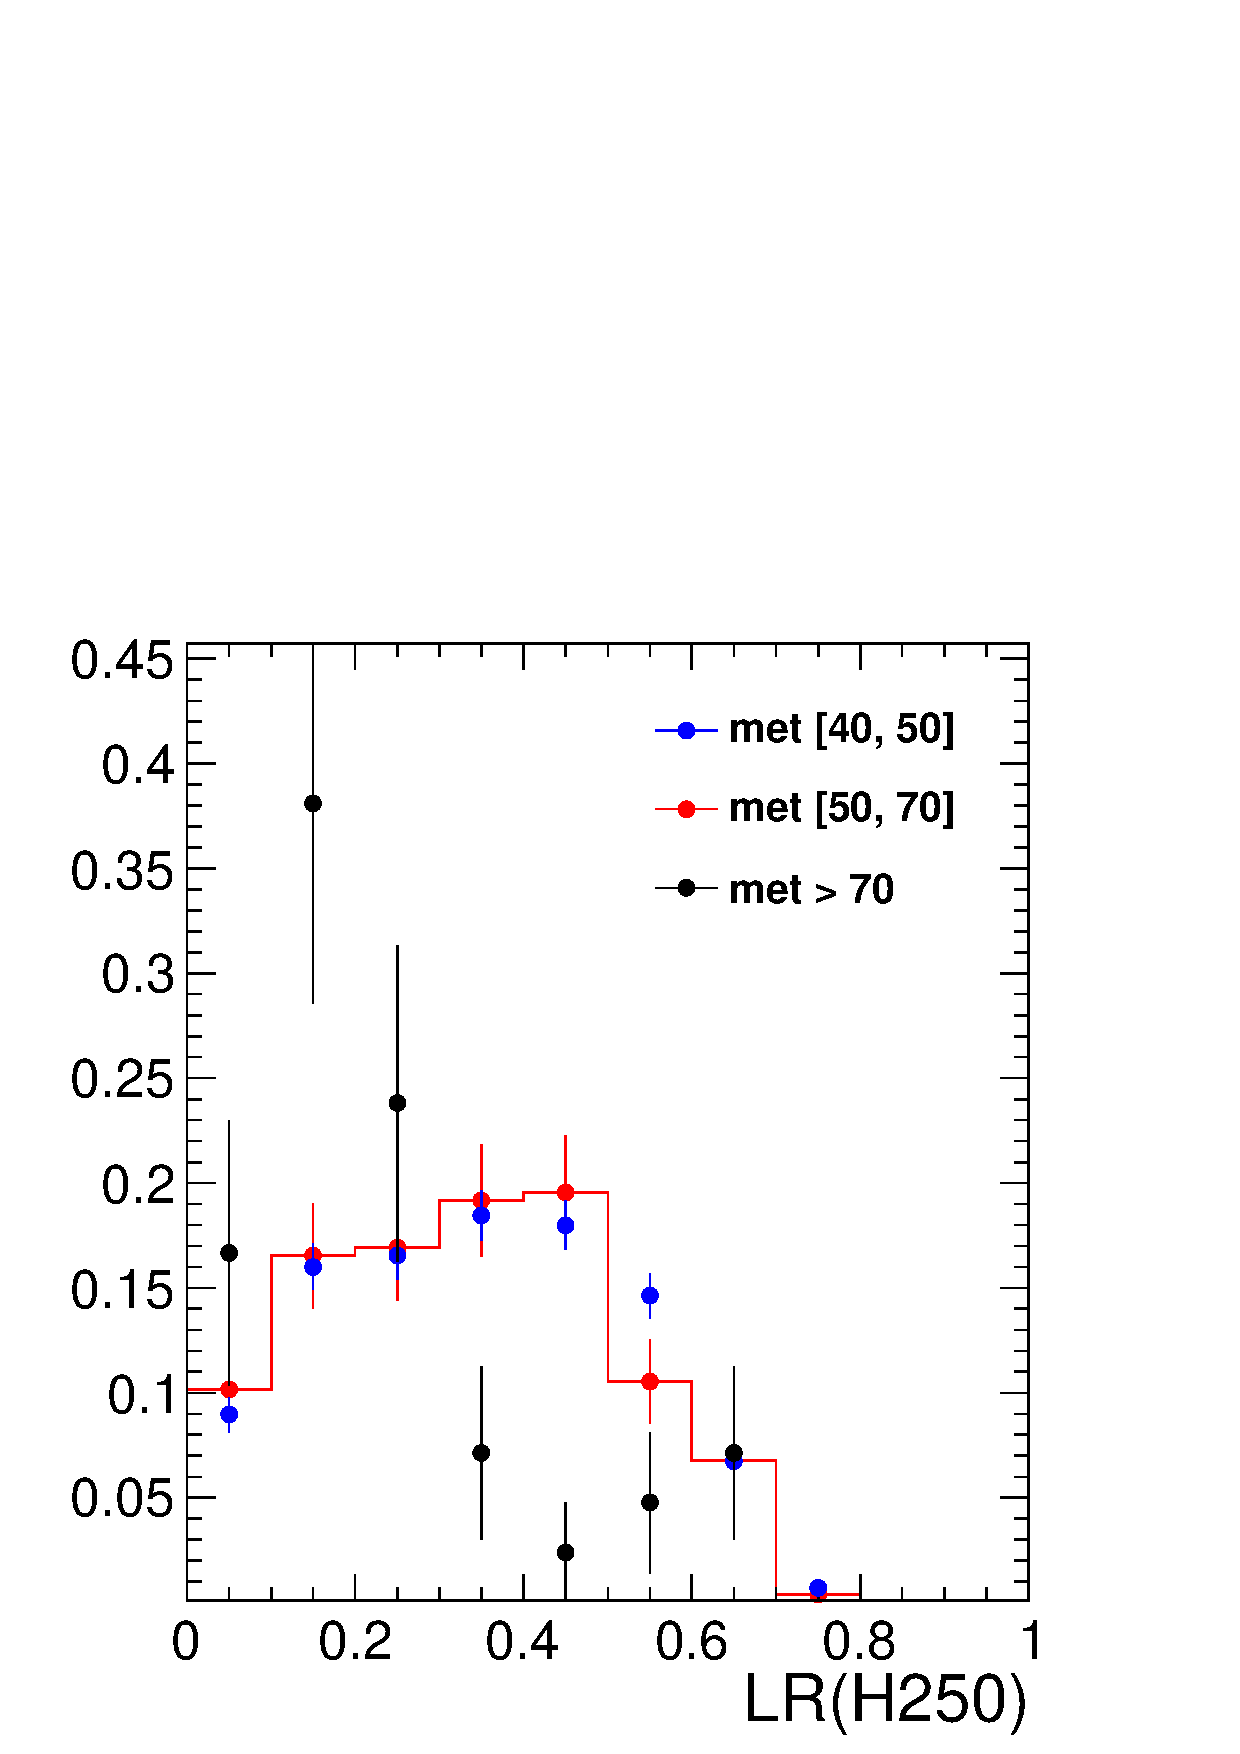
\includegraphics[width=.30\textwidth]{figures/Zee_LR_mH250_lin.png}         
\includegraphics[width=.30\textwidth]{figures/Zmm_LR_mH250_lin.png}} 
\subfigure[]{                                                                                                 
\centering                                                                                                    
\label{subfig:lr_met300}                                                                            
\includegraphics[width=.30\textwidth]{figures/Zee_LR_mH300_lin.png}         
\includegraphics[width=.30\textwidth]{figures/Zmm_LR_mH300_lin.png}}                                            
\subfigure[]{                                                                                                 
\centering                                                                                                    
\label{subfig:lr_met350}                                                                            
\includegraphics[width=.30\textwidth]{figures/Zee_LR_mH350_lin.png}         
\includegraphics[width=.30\textwidth]{figures/Zmm_LR_mH350_lin.png}}
\subfigure[]{                                                                                                 
\centering                                                                                                    
\label{subfig:lr_met400}                                                                            
\includegraphics[width=.30\textwidth]{figures/Zee_LR_mH400_lin.png}         
\includegraphics[width=.30\textwidth]{figures/Zmm_LR_mH400_lin.png}} 
\caption{Shape comparison of the matrix element output LR distribution in three \met regions for $Z$+jet Monte Carlo events, separately for $ee$ (left) and $\mu\mu$ (right) events. $m_H$~=~250, 300, 350 and 400 \GeVcc signal hypotheses are shown. The shapes are consistent within the uncertainties.}
\label{fig:LRshapeMET}                                                                                          
\end{figure}

\begin{figure}[!hbtp]                                                                                         
\centering  
\subfigure[]{                                                                                                 
\centering                                                                                                    
\label{subfig:lr_met250_datamc}
\includegraphics[width=.25\textwidth]{figures/Zee_LR_mH250_datamc_lin.png}         
\includegraphics[width=.25\textwidth]{figures/Zmm_LR_mH250_datamc_lin.png}} 
\subfigure[]{                                                                                                 
\centering                                                                                                    
\label{subfig:lr_met300_datamc}
\includegraphics[width=.25\textwidth]{figures/Zee_LR_mH300_datamc_lin.png}         
\includegraphics[width=.25\textwidth]{figures/Zmm_LR_mH300_datamc_lin.png}} 
\subfigure[]{                                                                                                 
\centering                                                                                                    
\label{subfig:lr_met350_datamc}
\includegraphics[width=.25\textwidth]{figures/Zee_LR_mH350_datamc_lin.png}         
\includegraphics[width=.25\textwidth]{figures/Zmm_LR_mH350_datamc_lin.png}} 
\subfigure[]{                                                                                                 
\centering                                                                                                    
\label{subfig:lr_met400_datamc}
\includegraphics[width=.25\textwidth]{figures/Zee_LR_mH400_datamc_lin.png}         
\includegraphics[width=.25\textwidth]{figures/Zmm_LR_mH400_datamc_lin.png}} 
\caption{Shape comparison of the matrix element output LR distribution in data and MC in $40<\met<50$ GeV region, separately for $ee$ (left) and $\mu\mu$ (right) events. $m_H$~=~250, 300, 350 and 400 \GeVcc signal hypotheses are shown. The shapes are consistent within the uncertainties.}
\label{fig:LRshapeMETDataMC}                                                                                          
\end{figure}


\subsection{Validation using $WZ+ZZ$ Cross-section Measurement}
\label{sec:vzvalidation}
We validate the performance of our implementation of the Matrix Element technique in $H\rightarrow ZZ$ by measuring
the $WZ+ZZ$ cross-section in events with two charged leptons and missing transverse energy. We perform this measurement
in dataset corresponding to 1.1 fb$^{-1}$ of integrated luminosity.
 
After the preselection cuts, the only relevant background in this measurement is non-resonant $WW$ production.
Therefore, the main challenge is to discriminate $ZZ$ and $WZ$ events from $WW$.
In order to achieve this, we construct a new likelihood $LR_{ZZ+WZ}$, defined as:
\begin{equation}
\label{eqn:LRZZ}
LR_{ZZ+WZ} = \frac { P_{ZZ}+P_{WZ}} { P_{ZZ} + P_{WZ} + P_{WW} },
\end{equation}
where $P_{WZ}$ is evaluated with the assumption that the two charged leptons originated from a $Z$-boson, while 
the $W$ decays leptonically but the lepton is not reconstructed. The distributions of LR$_{ZZ+WZ}$ for data and 
the predicted backgrounds and signal are shown in Figure \ref{fig:lrzz}. One can see that the shape of the distribution
in data is well-modeled.

%%%%%%%%%%%%%%%%%%%%%%%%%%%%%%
\begin{figure}[!htbp]
\begin{center}
\subfigure[]{                                                                                                 
\centering   
\label{subfig:lr_wzzz_ee}
\includegraphics[width=0.45\textwidth]{figures/ME_WZZZ_mH0_mm_stack_lin.png}}
\subfigure[]{                                                                                                 
\centering   
\label{subfig:lr_wzzz_mm}
\includegraphics[width=0.45\textwidth]{figures/ME_WZZZ_mH0_ee_stack_lin.png}}
\caption{$LR_{ZZ/WZ}$ in a 1.1 fb$^{-1}$ data sample compared to the expected backgrounds and the expected
$ZZ+WZ$ signal for $e-e$~\ref{subfig:lr_wzzz_mm} and $\mu-\mu$~\ref{subfig:lr_wzzz_ee} events. $ZZ$ and $WZ$ are shown twice, stacked and overlayed.}
\label{fig:lrzz}
\end{center}
\end{figure}
%%%%%%%%%%%%%%%%%%%%%%%%%%%%%%

A precise measurement of the cross-section requires a clean sample of signal events. We, therefore, further select events
that pass the requirement $LR_{ZZ+WZ}>0.75$.  The expected yields for each process as well as the observed data count
are  shown in Table~\ref{tab:ZZWZselection}.
Assuming a 100$\%$ systematic unceratainty on the backgrounds, we estimate the $ZZ+WZ$ 
cross-section to be $22.8 \pm 3.5$ pb, which is in agreement with theoretical predictions of $26.2$ pb.

\begin{table}[!hbtp]
  \begin{center}
  \begin{tabular} {c|c|c}
 \hline
  Process & $\mu-\mu$ events  & $e-e$ events \\
  \hline
  \hline
  $WW$                  &  0.2 $\pm$  0.1 &  0.2 $\pm$   0.1 \\
  $tt + tW$             &  0.6 $\pm$  0.1 &  0.1 $\pm$   0.1 \\
  $Z  + jets$           &  0.8 $\pm$  0.1 &  0.5 $\pm$   0.1\\
  $Z\rightarrow \tau\tau$& 0.0 $\pm$  0.1 &  0.0 $\pm$   0.1\\
  \hline
  Total Background      &  1.6 $\pm$  0.2 &  0.8 $\pm$   0.2\\
  \hline
  $ZZ$                  &  7.7 $\pm$  0.2 &  4.8 $\pm$   0.1\\
  $WZ$                  &  3.5  $\pm$ 0.1 &  1.9 $\pm$   0.1\\
 \hline
  Total Signal          &  11.2 $\pm$ 0.3 &  6.7 $\pm$   0.2\\
 \hline
  Data                  &  9               &   9              \\
 \hline
  \end{tabular}

  \caption{Expected number of signal and background events for a data sample with an 
  integrated luminosity of 1.1 fb$^{-1}$ after applying the $LR_{ZZ/WZ}>0.75$ requirement. 
 Uncertainties are statistical only.}
   \label{tab:ZZWZselection}
  \end{center}
\end{table}



\subsection{Results}
\label{sec:results_hzz}
The matrix element output (LR) are evaluated for six different values of $m_H$ between 250 and 600 \GeVcc.
Figure~\ref{fig:histo_me_250_5fb}-\ref{fig:histo_me_600_5fb} shows the matrix element output distributions 
comparing data to the signal and background predictions, corresponding to \intlumi data.

The observed and expected cross section ratio limits as a function of the Higgs mass, together with the 1/2-$\sigma$ uncertainty bands 
are shown in Table~\ref{tab:limits_5fb} and Figure~\ref{fig:limits_5fb} for these three analyses. 
%The corresponding $M_T$ and matrix element output distributions are shown in Appendix~\ref{app:mtshape} and Appendix~\ref{app:meshape} respectively.
Systematics uncertainties applied in the search are summarized in \cite{ref:HZZ2011smurf}.
Systematic variations affecting shapes of the likelihood ratio discriminant are included in the results presented in this note,
however methods to account for them are discussed separately in \cite{ref:ShapeSmurf}. 


With the current data sample, we expect to exclude the standard model Higgs boson 
in the mass range of about [300,450]~\GeVcc in the cut-based analysis, compared with the 
expected exclusion range of [300,475]~\GeVcc. 
The observed exclusion region extends to about [275-455]~\GeVcc using shape analysis based on 
$M_T$ variable, compared to the expected exclusion range of [290-490]~\GeVcc.
The observed exclusion region extends to about [300-500]~\GeVcc using shape analysis based on 
matrix element output, compared to the expected exclusion range of [280-480]~\GeVcc.

%%%%%%%%%%%%%%%%%%%%%%
\begin{figure}[!ht]
\begin{center}
   \subfigure[]{\includegraphics[width=0.4\textwidth,angle=0]{figures/ME_mH250_ee_stack_lin.pdf}} 
   \subfigure[]{\includegraphics[width=0.4\textwidth,angle=0]{figures/ME_mH250_mm_stack_lin.pdf}} \\ 
   \caption{The matrix element output distribution for Higgs signal and background events 
for \mHi=250 $\GeVcc$ in ee (a) and $\mu\mu$ final state (b) after the higgs dependent selections. 
The distributions are normalized to \intlumi with the background scaled by the data-to-mc ratios derived from data.}
   \label{fig:histo_me_250_5fb}
\end{center}
\end{figure}

\begin{figure}[!ht]
\begin{center}
   \subfigure[]{\includegraphics[width=0.4\textwidth,angle=0]{figures/ME_mH300_ee_stack_log.pdf}} 
   \subfigure[]{\includegraphics[width=0.4\textwidth,angle=0]{figures/ME_mH300_mm_stack_log.pdf}} \\ 
   \caption{The matrix element output distribution for Higgs signal and background events 
for \mHi=300 $\GeVcc$ in ee (a) and $\mu\mu$ final state (b) after the higgs dependent selections. 
The distributions are normalized to \intlumi with the background scaled by the data-to-mc ratios derived from data.}
   \label{fig:histo_me_300_5fb}
\end{center}
\end{figure}

\begin{figure}[!ht]
\begin{center}
   \subfigure[]{\includegraphics[width=0.4\textwidth,angle=0]{figures/ME_mH350_ee_stack_log.pdf}} 
   \subfigure[]{\includegraphics[width=0.4\textwidth,angle=0]{figures/ME_mH350_mm_stack_log.pdf}} \\ 
   \caption{The matrix element output distribution for Higgs signal and background events 
for \mHi=350 $\GeVcc$ in ee (a) and $\mu\mu$ final state (b) after the higgs dependent selections. 
The distributions are normalized to \intlumi with the background scaled by the data-to-mc ratios derived from data.}
   \label{fig:histo_me_350_5fb}
\end{center}
\end{figure}

\begin{figure}[!ht]
\begin{center}
   \subfigure[]{\includegraphics[width=0.4\textwidth,angle=0]{figures/ME_mH400_ee_stack_log.pdf}} 
   \subfigure[]{\includegraphics[width=0.4\textwidth,angle=0]{figures/ME_mH400_mm_stack_log.pdf}} \\ 
   \caption{The matrix element output distribution for Higgs signal and background events 
for \mHi=400 $\GeVcc$ in ee (a) and $\mu\mu$ final state (b) after the higgs dependent selections. 
The distributions are normalized to \intlumi with the background scaled by the data-to-mc ratios derived from data.}
   \label{fig:histo_me_400_5fb}
\end{center}
\end{figure}


\begin{figure}[!ht]
\begin{center}
   \subfigure[]{\includegraphics[width=0.4\textwidth,angle=0]{figures/ME_mH500_ee_stack_log.pdf}} 
   \subfigure[]{\includegraphics[width=0.4\textwidth,angle=0]{figures/ME_mH500_mm_stack_log.pdf}} \\ 
   \caption{The matrix element output distribution for Higgs signal and background events 
for \mHi=500 $\GeVcc$ in ee (a) and $\mu\mu$ final state (b) after the higgs dependent selections. 
The distributions are normalized to \intlumi with the background scaled by the data-to-mc ratios derived from data.}
   \label{fig:histo_me_500_5fb}
\end{center}
\end{figure}

\begin{figure}[!ht]
\begin{center}
   \subfigure[]{\includegraphics[width=0.4\textwidth,angle=0]{figures/ME_mH600_ee_stack_log.pdf}} 
   \subfigure[]{\includegraphics[width=0.4\textwidth,angle=0]{figures/ME_mH600_mm_stack_log.pdf}} \\ 
   \caption{The matrix element output distribution for Higgs signal and background events 
for \mHi=600 $\GeVcc$ in ee (a) and $\mu\mu$ final state (b) after the higgs dependent selections. 
The distributions are normalized to \intlumi with the background scaled by the data-to-mc ratios derived from data.}
   \label{fig:histo_me_600_5fb}
\end{center}
\end{figure}
%%%%%%%%%%%%%%%%%%%%%%




%%%%%%%%%%%%%%%%%%%%%%%%%%%%%%%
\begin{table}[!htbp]
\begin{center}
\begin{tabular}{ccccc}
\hline\hline
Mass & Observed & Median Expected & [-$\sigma$, +$\sigma$] & [-2$\sigma$, +2$\sigma$]\\\hline
\hline
\multicolumn{5}{c} {Cut-based Analysis} \\ 
\hline
250 & 1.62 & 1.62 & [1.17, 2.24] & [0.88, 2.98] \\
300 & 0.95 & 1.04 & [0.75, 1.44] & [0.56, 1.91] \\
350 & 0.60 & 0.68 & [0.49, 0.94] & [0.37, 1.25] \\
400 & 0.59 & 0.65 & [0.47, 0.91] & [0.35, 1.21] \\
500 & 1.61 & 1.19 & [0.86, 1.66] & [0.65, 2.20] \\
600 & 2.20 & 2.36 & [1.70, 3.28] & [1.28, 4.36] \\
\hline
\multicolumn{5}{c} {Shape Analysis Based on $M_T$} \\ 
\hline
250 & 1.50 & 1.38 & [1.00, 1.92] & [0.75, 2.56] \\
300 & 0.66 & 0.93 & [0.67, 1.29] & [0.51, 1.72] \\
350 & 0.55 & 0.63 & [0.45, 0.87] & [0.34, 1.16] \\
400 & 0.54 & 0.63 & [0.46, 0.88] & [0.34, 1.17] \\
500 & 1.58 & 1.08 & [0.78, 1.50] & [0.58, 1.99] \\
600 & 2.41 & 2.23 & [1.61, 3.10] & [1.21, 4.12] \\
\hline
\multicolumn{5}{c} {Shape Analysis Based on Matrix Element Output} \\ 
\hline
250 & 1.20 & 1.31 & [0.95, 1.83] & [0.71, 2.43] \\
300 & 0.99 & 0.87 & [0.63, 1.21] & [0.47, 1.60] \\
350 & 0.63 & 0.64 & [0.46, 0.88] & [0.35, 1.18] \\
400 & 0.56 & 0.64 & [0.46, 0.89] & [0.35, 1.19] \\
500 & 0.99 & 1.13 & [0.82, 1.57] & [0.61, 2.09] \\
600 & 1.96 & 2.43 & [1.75, 3.37] & [1.32, 4.48] \\
\hline\hline
\end{tabular}
\end{center}
\caption{The observed and expected cross section ratio limits as a function 
of the Higgs mass, together with the 1/2-$\sigma$ uncertainty bands obtained in the cut-and-count analysis 
and shape analyses based on both $M_T$ variable and matrix element output.
The limits correspond to an integrated luminosity of \intlumi, shown in Figure~\ref{fig:limits_5fb}.}
\label{tab:limits_5fb}
\end{table}
%%%%%%%%%%%%%%%%%%%%%%%%%%%%%



%%%%%%%%%%%%%%%%%%%%%%%%%%%%%
\begin{figure}[!htbp]
  \begin{center}
  \subfigure[Cut-based Analysis]{
  \label{subfig:cutbased}
  \includegraphics[width=0.5\textwidth]{figures/limits_cut_5fb.pdf}} \\
\end{center}
  \subfigure[$M_T$ Shape Analysis]{
  \centering
  \label{subfig:mtshape}
   \includegraphics[width=0.5\textwidth]{figures/limits_mtshape_5fb.pdf}}
  \subfigure[Matrix Element Shape Analysis]{
  \centering
  \label{subfig:meshape}
   \includegraphics[width=0.5\textwidth]{figures/limits_meshape_5fb.pdf}}
\caption{The observed and expected upper limits at 95\% C.L. for \intlumi\ of data for the 
	cut-based analysis \subref{subfig:cutbased} and 
	shape analyses based on both $M_T$ variable \subref{subfig:mtshape} 
	and matrix element output \subref{subfig:meshape} The values are 
	tabulated in Table~\ref{tab:limits_5fb}.  
}	
\label{fig:limits_5fb}
\end{figure}
%%%%%%%%%%%%%%%%%%%%%%%%%%%%%

\clearpage


\section{Summary}
\label{sec:summary}
In summary, we described an analysis to study the spin of a single narrow 
resonance at 125 GeV by the gluon fusion through the decays into $WW\to 2\ell2\nu$.  
The analysis is based on a two-dimensional templates $m_T-m_{\ell\ell}$. 
The expected sensitivity to distinguish between between SM Higgs hypothesis and 
spin 2 Graviton like resonance with minimal coupling 
$2_\text{min}^+$ is $1.7\sigma$ for \intlumiEightTeV. 
Scaling by luminosity the projected separation is about $2.0\sigma$ for 25~$\ifb$. 


\clearpage

\appendix


 \section{$H\to WW$ expected and observed upper limits by sub-channels}
     \label{app:hwwsubchannels}
     In this section we tabulated the observed and expected upper limits 
in $H\to WW$ analysis in different sub-channels, corresponding to the 
results shown in Figure~\ref{fig:me_results_5fb_subchannel}.

%%%%%%%%%%%%%%%%%%%%%%%%%%%%%%
\begin{table}[!htbp]
\begin{center}
\begin{tabular}{c c c c c c}
\hline\hline
 Higgs Mass   & Observed & Median expected & Expected range for 68\% & Expected range for 95\%   \\
\hline
\multicolumn{5}{c} {BDT Based} \\
\hline
115 & 6.1 & 7.8 & [5.3, 11.9] & [3.8, 18.3] \\
120 & 3.5 & 4.0 & [2.7, 6.1] & [1.9, 9.1] \\
130 & 1.4 & 1.5 & [1.0, 2.2] & [0.7, 3.3] \\
140 & 0.8 & 0.9 & [0.6, 1.3] & [0.4, 1.8] \\
150 & 0.8 & 0.6 & [0.4, 0.9] & [0.3, 1.3] \\
160 & 0.5 & 0.3 & [0.2, 0.4] & [0.1, 0.6] \\
170 & 0.4 & 0.3 & [0.2, 0.5] & [0.2, 0.7] \\
180 & 0.6 & 0.5 & [0.3, 0.7] & [0.2, 1.0] \\
190 & 0.9 & 0.7 & [0.5, 1.0] & [0.3, 1.5] \\
200 & 1.3 & 1.0 & [0.7, 1.5] & [0.5, 2.3] \\
250 & 2.2 & 2.1 & [1.4, 3.1] & [1.0, 4.3] \\
\hline
\multicolumn{5}{c} {Matrix Element Method} \\
\hline
115 & 4.1 & 7.6 & [5.1, 12.3] & [3.6, 19.2] \\
120 & 2.8 & 4.3 & [2.8, 6.2] & [2.0, 9.3] \\
130 & 1.3 & 1.6 & [1.1, 2.4] & [0.7, 3.6] \\
140 & 0.9 & 1.0 & [0.7, 1.5] & [0.4, 2.2] \\
150 & 0.7 & 0.6 & [0.4, 0.9] & [0.3, 1.3] \\
160 & 0.4 & 0.3 & [0.2, 0.4] & [0.1, 0.6] \\
170 & 0.3 & 0.3 & [0.2, 0.5] & [0.1, 0.7] \\
180 & 0.5 & 0.4 & [0.3, 0.6] & [0.2, 0.9] \\
190 & 0.7 & 0.7 & [0.5, 1.0] & [0.3, 1.5] \\
200 & 1.1 & 0.9 & [0.6, 1.4] & [0.4, 2.0] \\
250 & 1.6 & 1.9 & [1.3, 2.9] & [0.9, 4.4] \\
\hline\hline
\end{tabular}
\end{center}
\caption{Multivariate shape analysis expected and observed upper limits at 95\% C.L.
for $\intlumi$ data using the BDT and matrix element outputs for the 
{\bf 0 jet bin same flavor final state}.}
\label{tab:me_results_5fb_0jsf}
\end{table}
%%%%%%%%%%%%%%%%%%%%%%%%%%%%%%


%%%%%%%%%%%%%%%%%%%%%%%%%%%%%%
\begin{table}[!htbp]
\begin{center}
\begin{tabular}{c c c c c c}
\hline\hline
 Higgs Mass   & Observed & Median expected & Expected range for 68\% & Expected range for 95\%   \\
\hline
\multicolumn{5}{c} {BDT Based} \\
\hline
115 & 4.5 & 3.6 & [2.6, 5.3] & [1.8, 8.3] \\
120 & 2.9 & 2.1 & [1.5, 3.2] & [1.0, 4.6] \\
130 & 1.1 & 1.0 & [0.7, 1.5] & [0.5, 2.1] \\
140 & 0.8 & 0.6 & [0.4, 0.9] & [0.3, 1.4] \\
150 & 0.5 & 0.4 & [0.3, 0.6] & [0.2, 0.9] \\
160 & 0.4 & 0.2 & [0.2, 0.4] & [0.1, 0.5] \\
170 & 0.4 & 0.3 & [0.2, 0.4] & [0.1, 0.6] \\
180 & 0.4 & 0.4 & [0.3, 0.6] & [0.2, 0.9] \\
190 & 0.7 & 0.6 & [0.4, 1.0] & [0.3, 1.4] \\
200 & 1.0 & 0.9 & [0.6, 1.4] & [0.4, 2.1] \\
250 & 1.4 & 1.7 & [1.1, 2.6] & [0.7, 3.9] \\
\hline
\multicolumn{5}{c} {Matrix Element Method} \\
\hline
115 & 3.6 & 3.8 & [2.5, 5.4] & [1.8, 7.9] \\
120 & 2.9 & 2.3 & [1.6, 3.4] & [1.1, 5.0] \\
130 & 1.3 & 1.1 & [0.8, 1.6] & [0.5, 2.4] \\
140 & 1.3 & 0.7 & [0.4, 1.0] & [0.3, 1.5] \\
150 & 0.7 & 0.5 & [0.3, 0.7] & [0.2, 0.9] \\
160 & 0.3 & 0.2 & [0.2, 0.3] & [0.1, 0.5] \\
170 & 0.4 & 0.3 & [0.2, 0.4] & [0.1, 0.5] \\
180 & 0.4 & 0.4 & [0.2, 0.6] & [0.2, 0.8] \\
190 & 0.6 & 0.6 & [0.4, 0.9] & [0.3, 1.3] \\
200 & 1.1 & 0.8 & [0.6, 1.2] & [0.4, 1.7] \\
250 & 1.3 & 1.5 & [1.0, 2.2] & [0.7, 3.4] \\
\hline\hline
\end{tabular}
\end{center}
\caption{Multivariate shape analysis expected and observed upper limits at 95\% C.L.
for $\intlumi$ data using the BDT and matrix element outputs for the 
{\bf 0 jet bin opposite flavor final state}.}
\label{tab:me_results_5fb_0jof}
\end{table}
%%%%%%%%%%%%%%%%%%%%%%%%%%%%%%



%%%%%%%%%%%%%%%%%%%%%%%%%%%%%%
\begin{table}[!htbp]
\begin{center}
\begin{tabular}{c c c c c c}
\hline\hline
 Higgs Mass   & Observed & Median expected & Expected range for 68\% & Expected range for 95\%   \\
\hline
\multicolumn{5}{c} {BDT Based} \\
\hline
115 & 17.4 & 19.5 & [13.5, 28.7] & [9.7, 42.2] \\
120 & 9.7 & 9.4 & [6.3, 14.0] & [4.7, 19.5] \\
130 & 4.5 & 3.2 & [2.2, 4.8] & [1.6, 6.9] \\
140 & 2.6 & 1.6 & [1.1, 2.4] & [0.8, 3.4] \\
150 & 1.4 & 1.0 & [0.7, 1.5] & [0.5, 2.2] \\
160 & 0.9 & 0.6 & [0.4, 0.9] & [0.3, 1.2] \\
170 & 0.9 & 0.6 & [0.4, 0.9] & [0.3, 1.3] \\
180 & 0.8 & 0.8 & [0.5, 1.1] & [0.4, 1.6] \\
190 & 1.5 & 1.3 & [0.9, 1.9] & [0.6, 2.7] \\
200 & 2.5 & 1.8 & [1.2, 2.7] & [0.8, 4.0] \\
250 & 6.0 & 3.5 & [2.4, 5.4] & [1.7, 8.2] \\
\hline
\multicolumn{5}{c} {Matrix Element Method} \\
\hline
115 & 18.0 & 19.9 & [13.2, 29.4] & [9.2, 44.6] \\
120 & 10.9 & 9.2 & [6.5, 13.9] & [4.7, 21.7] \\
130 & 5.5 & 3.8 & [2.5, 5.8] & [1.7, 8.6] \\
140 & 2.5 & 1.9 & [1.3, 2.9] & [0.9, 4.2] \\
150 & 1.3 & 1.1 & [0.7, 1.6] & [0.5, 2.3] \\
160 & 0.9 & 0.6 & [0.4, 1.0] & [0.3, 1.4] \\
170 & 0.8 & 0.7 & [0.5, 1.0] & [0.3, 1.4] \\
180 & 0.7 & 0.9 & [0.6, 1.3] & [0.4, 2.0] \\
190 & 1.1 & 1.4 & [1.0, 2.1] & [0.6, 3.0] \\
200 & 1.8 & 2.0 & [1.3, 3.1] & [0.8, 4.6] \\
250 & 6.7 & 3.9 & [2.6, 6.1] & [1.8, 9.3] \\
\hline\hline
\end{tabular}
\end{center}
\caption{Multivariate shape analysis expected and observed upper limits at 95\% C.L.
for $\intlumi$ data using the BDT and matrix element outputs for the 
{\bf 1 jet bin same flavor final state}.}
\label{tab:me_results_5fb_1jsf}
\end{table}
%%%%%%%%%%%%%%%%%%%%%%%%%%%%%%



%%%%%%%%%%%%%%%%%%%%%%%%%%%%%%
\begin{table}[!htbp]
\begin{center}
\begin{tabular}{c c c c c c}
\hline\hline
 Higgs Mass   & Observed & Median expected & Expected range for 68\% & Expected range for 95\%   \\
\hline
\multicolumn{5}{c} {BDT Based} \\
\hline
115 & 13.7 & 6.2 & [4.3, 9.5] & [3.0, 13.8] \\
120 & 7.1 & 3.6 & [2.5, 5.3] & [1.7, 8.0] \\
130 & 2.8 & 1.7 & [1.1, 2.5] & [0.8, 3.4] \\
140 & 1.4 & 1.0 & [0.7, 1.5] & [0.5, 2.1] \\
150 & 1.0 & 0.7 & [0.5, 1.1] & [0.3, 1.7] \\
160 & 0.4 & 0.5 & [0.3, 0.7] & [0.2, 1.0] \\
170 & 0.5 & 0.5 & [0.3, 0.7] & [0.2, 1.1] \\
180 & 0.5 & 0.7 & [0.4, 1.0] & [0.3, 1.5] \\
190 & 0.7 & 1.1 & [0.7, 1.6] & [0.5, 2.5] \\
200 & 1.2 & 1.5 & [1.0, 2.2] & [0.7, 3.5] \\
250 & 2.2 & 2.8 & [1.8, 4.3] & [1.2, 6.2] \\
\hline
\multicolumn{5}{c} {Matrix Element Method} \\
\hline
115 & 13.4 & 7.6 & [5.1, 11.9] & [3.5, 18.2] \\
120 & 6.2 & 4.2 & [2.8, 6.3] & [1.9, 9.8] \\
130 & 2.4 & 1.9 & [1.3, 2.9] & [0.8, 4.4] \\
140 & 1.5 & 1.1 & [0.7, 1.7] & [0.5, 2.5] \\
150 & 1.2 & 0.8 & [0.5, 1.2] & [0.4, 1.8] \\
160 & 0.5 & 0.5 & [0.3, 0.7] & [0.2, 1.0] \\
170 & 0.4 & 0.5 & [0.3, 0.8] & [0.2, 1.1] \\
180 & 0.6 & 0.7 & [0.4, 1.0] & [0.3, 1.5] \\
190 & 0.9 & 1.1 & [0.7, 1.6] & [0.5, 2.3] \\
200 & 1.5 & 1.6 & [1.0, 2.4] & [0.6, 3.5] \\
250 & 2.5 & 2.7 & [1.8, 4.1] & [1.2, 5.9] \\
\hline\hline
\end{tabular}
\end{center}
\caption{Multivariate shape analysis expected and observed upper limits at 95\% C.L.
for $\intlumi$ data using the BDT and matrix element outputs for the 
{\bf 1 jet bin opposite flavor final state}.}
\label{tab:me_results_5fb_1jof}
\end{table}
%%%%%%%%%%%%%%%%%%%%%%%%%%%%%%




\clearpage

\vspace*{-0.2cm}
\thebibliography{12}

\bibitem{pdg}
 K. Nakamura et al. (Particle Data Group), "Review of particle physics", J. Phys.G37 , 2010.

\bibitem{Higgs1}
F. Englert and R. Brout, "Broken symmetries and the masses of gauge bosons", Phys. Rev. Lett. 13,  1964.

\bibitem{Higgs2}
P. W. Higgs, "Broken symmetry and the mass of gauge vector mesons", Phys. Rev. Lett. 13, 1964.

\bibitem{Higgs3}
Guralnik, G.S. and Hagen, C.R. and Kibble, T.W.B., "Global Conservation Laws and Massless Particles", 
Phys.Rev.Lett. 13, 1964.

\bibitem{HWW2010}
CMS Collaboration, "Title: Measurement of WW Production and Search for the Higgs Boson in 
pp Collisions at $\sqrt{s}$ = 7 TeV", arXiv:1102.5429

\bibitem{VBTFCrossSectionNote}
J. Alcaraz Maestre, \textit{et al.}, "Updated Measurements of Inclusive W and Z Cross Sections 
at $\sqrt{s}=7$ TeV", CMS AN-2010/264.

\bibitem{ggWWError}
F.~ Stoeckli, "http://indico.cern.ch/getFile.py/access?contribId=0\&resId=1\&materialId=slides\&confId=49009", 
EWK Diboson meeting of March 12 2009.

\bibitem{json}
{\small
/afs/cern.ch/cms/CAF/CMSCOMM/COMM\_DQM/certification/Collisions11/7TeV/Prompt/Cert\_160404-163869\_7TeV\_PromptReco\_Collisions11\_JSON.txt
}

\bibitem{ElIso}
A. Vartak, M. LeBourgeois, V. Sharma, "Lepton Isolation in the CMS Tracker, ECAL and HCAL", CMS AN-2010/106.

\bibitem{PVDA}
W. Erdmann, M. LeBourgeois, B. Mangano, 
https://indico.cern.ch/getFile.py/access?contribId=5\&sessionId=3\&resId=1\&materialId=slides\&confId=127127, 
note in preparation.

\bibitem{NExpHits}
B. Mangano \textit{et al.}, "Improvement in Photon Conversion Rejection Performance Using 
Advanced Tracking Tools", AN-10-283.

\bibitem{fakeLeptonNote1}
S.~Xie, \textit{et al.}", "Study of Data-Driven Methods for Estimation of Fake Lepton Backgrounds", 
CMS AN-2009/120.

\bibitem{fakeLeptonNote2}
W.~Andrews, \textit{et al.}, "Fake Rates for dilepton Analyses", CMS AN-2010/257.

\bibitem{fakeLeptonBkgSpillage1}
 F. Golf, D. Evans, J. Mulmenstadt  \textit{et al.}, ``Expectations for observation of top quark pair production in the dilepton final state with the early CMS data'', CMS AN-2009/050.

\bibitem{dyestnote}
W. Andrews, et al., “A Method to Measure the Contribution of $\dyll$ to a di-lepton+ MET Selection”, CMS AN-2009/023 (2009).

\bibitem{jes}
CMS Collaboration, "Jet Energy Calibration with Photon+Jet Events", PAS JME-09-004.

\bibitem{jetpas}
CMS Collaboration, "Jet Performance in pp Collisions at $\sqrt{s}=7 \rm\ TeV$", PAS JME-10-003.

\bibitem{btag}
CMS collaboration, "Commissioning of b-jet identification with pp collisions at $\sqrt{s}=7~\TeV$, BTV-10-001.

\bibitem{antikt}
Cacciari, Matteo and Salam, Gavin P. and Soyez, Gregory, "The anti-$k_t$ jet clustering 
algorithm", JHEP 04,  2008.

\bibitem{ConversionNote}
W.~Andrews, \textit{et al.}, "Study of photon conversion rejection at CMS", CMS AN-2009/159.

\bibitem{tmva}
A. Hoecker, \textit{et al.}, "TMVA - Toolkit for Multivariate Data Analysis", arXiv:physics/0703039, 2007.

\bibitem{XS}
CMS Generator group, Standard Model Cross Sections for CMS at 7 TeV, 2010.

\bibitem{PDF4LHC}
PDF4LHC Working Group, 
{\tt http://www.hep.ucl.ac.uk/pdf4lhc/PDF4LHCrecom.pdf}

\bibitem{Nadolsky:2008zw}
Nadolsky, Pavel M. and others, "Implications of CTEQ global analysis for 
collider observables", Phys. Rev. D78 2008.

\bibitem{Martin:2009iq}
Martin, A. D. and Stirling, W. J. and Thorne, R. S. and Watt, G., "Parton 
distributions for the LHC, Eur. Phys. J. C63 2009.

\bibitem{Ball:2010de}
Ball, Richard D. and others, "A first unbiased global NLO determination 
of parton distributions and their uncertainties", arXiv 1002.4407.

\bibitem{bayesian}
A. O'Hagan and J.J. Forster, "Bayesian Inference", Kendall's Advanced Theory of Statistics, 
Arnold, London, 2B, 2004.

\bibitem{ref:tagprobe_mit_w}
G. Bauer {\it et. al.}, "Lepton ef?iencies for the inclusive W cross section measurement with 36.1pb$^{-1}$", AN2011/097

\bibitem{ref:tagprobe_snt_top}
W. Andrews {\it et. al.}, "Uncertainties on the Lepton Selection Efficiency for t$t\bar{t}$ Cross Section Analysis", AN2010/274

\bibitem{LHCHiggsCrossSectionWorkingGroup:2011ti}
LHC Higgs Cross Section Working Group, "Handbook of LHC Higgs Cross Sections: 
Inclusive Observables", CERN-2011-002, 2011.

\bibitem{PFMET} 
CMS Collaboration, ``CMS MET Performance in Events Containing Electroweak Bosons from pp Collisions at $\sqrt{s}=7$ TeV'', CMS PAS JME-2010-005 (2010)


\bibitem{trkMET} 
Marco Zanetti, ``MET with PU in $\hww\to2\ell$'', https://indico.cern.ch/conferenceDisplay.py?confId=131580
Benjamin Hooberman, ``MET with PU in MC and First 2011 Data'', https://indico.cern.ch/contributionDisplay.py?contribId=5\&confId=132579. 


\bibitem{lands}
Mingshui Chen and Andrey Korytov, https://mschen.web.cern.ch/mschen/lands/

\bibitem{MCFMHiggsProduction}
J. Campbell, R.K. Ellis, G. Zanderighi, ``Next-to-Leading order Higgs + 2 jet production via gluon fusion.'', JHEP 0610:028 (2006), hep-ph/0608194 




\end{document}
